%!TEX root=../main.tex
\chapter{Results and Discussion}%keine interpretation
\acresetall %reset abbrevations
\label{chap:results}


In this chapter, we present the findings from the experimental evaluation, and address the core research questions systematically.
The overall goal of these experiments was to provide a fair comparison of deep learning models, kinematic models, and stochastic filters, as well as to investigate the impact of incorporating geographic domain information into model training and architecture.
To evaluate the three research questions outlined in Section \ref{sec:rqand}, we conducted a total of three experiments: a baseline comparison of all motion models on the full dataset (Exp I), an assessment of the effect of domain-specific training on predictive performance (Exp II), and an ablation study of explicit domain encoding for LSTMs (Exp III).
The remainder of this chapter is structured around the  questions, for each of which we present the quantitative results first, along with the answers to our research questions. A more detailed discussion of the results follows.

The preprocessed dataset is provided at Hugging Face\footnote{\url{https://huggingface.co/datasets/kawihss/ais-inland-vessel-trajectories}}. 
The dataset can be regenerated with the pipeline provided at RWTH GitLab\footnote{\url{https://git-ce.rwth-aachen.de/g-nav-mob-irt/projects/galileonautic2plus/multi-object-tracking/motion-models/-/tree/handedIn}} or the public GitHub mirror\footnote{\url{https://github.com/kawihss/Data-based-vessel-motion-modelling-Thesis/tree/handedIn}}. 
The repository also provides the code to train and optimise all models. For details on the pipeline, refer to the readme files and Appendix~\ref{chap:appendixcodebase} for a general overview of the codebase architecture.

%\section[Exp. \Romannum{1}: Motion Model Comparison]{Exp. \Romannum{1}: Baseline Comparison of Motion Models} 

 
\textbf{RQ 1:} \textit{Given a preprocessed dataset and a systematic hyperparameter optimisation procedure, how do deep learning models, both task-specific and pretrained, kinematic baselines, and stochastic filters compare in short-term trajectory prediction of inland vessels?}

We set up Exp. \Romannum{1} to answer this question and to serve as an overall baseline comparison across all evaluated motion models and model families on the full dataset. 

\paragraph{Results.}
The optimised hyperparameter configurations for all evaluated models are listed in Table~\ref{tab:hpo_results_exp0}, and the corresponding test set error metrics are detailed in Table~\ref{tab:results_exp0}.
Specifically, the standard \ac{LSTM} achieves an \ac{ADE} of $54.78$\,m and a \acf{RMSE} of $111.36$\,m, reducing the error of the \ac{CV} baseline (\ac{ADE} $78.39$\,m, \ac{RMSE} $155.73$\,m) by $30.1\%$ and $28.5\%$, respectively.
To assess the overall statistical significance of these results, we conducted a Friedman test combined with Nemenyi post-hoc comparison.
The significant differences are illustrated as a \ac{CD} diagram in Figure~\ref{fig:cd_test}. 
The diagram reveals a clear ranking structure: the two LSTM-based models occupy the top positions, with average ranks of 1.5 and 2 respectively, followed by the \ac{EKF} (4.7) and Chronos-2 (5.4), while the remaining models form a middle group with mostly non-significant pairwise differences (6.4 -- 7).
The CTRV-based models rank last (8.1).



\begin{table}[t]
%\centering
\noindent
\caption[Exp. I Optimised Hyperparameter Configurations]{Optimised hyperparameter (HP) configurations for all models. Discussed parameters are shaded.}
\label{tab:hpo_results_exp0}
\begin{minipage}[t]{0.49\textwidth}
\centering
\begin{tabular}{llr}
\toprule
\textbf{Model} & \textbf{HP} & \textbf{Value} \\
\midrule
CV             & \cellcolor{blue!15}$n_\text{vel}$  & \cellcolor{blue!15}1 \\
CTRV           & $n_\text{vel}$                     & 2 \\
CTRV Arc       & $n_\text{vel}$                     & 3 \\
Hybrid         & $n_\text{vel}^\text{CV}$            & 1 \\
               & $n_\text{vel}^\text{CTRV}$          & 2 \\
               & $n_\text{rot}$                      & 1 \\
               & \cellcolor{blue!15}$\tau_\text{rot}$& \cellcolor{blue!15}29.28°/min \\
\midrule
KF (CV)        & \cellcolor{cyan!15}$q_\text{pos}$  & \cellcolor{cyan!15}$1.578{\times}10^{-3}$ \\
               & $q_\text{vel}$                     & $5.932$ \\
               & \cellcolor{cyan!15}$r_\text{pos}$  & \cellcolor{cyan!15}$1.077{\times}10^{-2}$ \\
               & $p_{0,\text{pos}}$                 & $7.737{\times}10^{-2}$ \\
               & $p_{0,\text{vel}}$                 & $1.190{\times}10^{-1}$ \\
\midrule
EKF (CTRV)     & \cellcolor{green!15}$q_\text{pos}$ & \cellcolor{green!15}$15.957$ \\
               & $q_\text{vel}$                     & $4.290{\times}10^{-2}$ \\
               & \cellcolor{green!15}$q_\text{rot}$ & \cellcolor{green!15}$1.002{\times}10^{-7}$ \\
               & $r_\text{pos}$                     & $1.792{\times}10^{-2}$ \\
               & $p_{0,\text{pos}}$                 & $4.046{\times}10^{-1}$ \\
               & $p_{0,\text{vel}}$                 & $1.845{\times}10^{-3}$ \\
               & $p_{0,\text{rot}}$                 & $2.076{\times}10^{-6}$ \\
               & $n_\text{ctx}$                     & 2 \\
\bottomrule
\end{tabular}
\end{minipage}
%\hfill
\begin{minipage}[t]{0.40\textwidth}
\centering
\begin{tabular}{llr}
\toprule
\textbf{Model} & \textbf{HP} & \textbf{Value} \\
\midrule
Chronos-2      & \multicolumn{2}{l}{\textit{no HPO}} \\
TiRex          & context length          & 1 \\
\midrule
LSTM           & hidden size             & 256 \\
               & num.\ layers            & 2 \\
               & dropout                 & 0.290 \\
               & learning rate           & $5.530{\times}10^{-4}$ \\
               & batch size              & 128 \\
               & \cellcolor{orange!15}feature set & \cellcolor{orange!15}no rot \\
\midrule
LSTM+Domain    & hidden size             & 256 \\
               & num.\ layers            & 2 \\
               & dropout                 & 0.300 \\
               & learning rate           & $4.000{\times}10^{-4}$ \\
               & batch size              & 256 \\
               & feature set             & all \\
\bottomrule
\end{tabular}
\end{minipage}
\end{table}


\begin{table}[t]
\centering
\caption[Exp. I Test Set Error Metrics] {Test set error metrics for all models}%Discussed metrics shaded in.}
\label{tab:results_exp0}
\begin{tabular}{lrrr}
\toprule
\textbf{Model} & \textbf{ADE} & \textbf{FDE} & \textbf{RMSE} \\
\midrule
CV                  & 78.39 & 175.82 & 155.73 \\
CTRV                & 82.92 & 195.18 & 164.51 \\
CTRV Arc            & 85.21 & 196.78 & 168.29 \\
Hybrid CV/CTRV      & 78.49 & 176.45 & 155.49 \\
\midrule
KF (CV)             & 78.39 & 175.82 & 155.73 \\
EKF (CTRV)          & 78.94 & 174.88 & 151.50 \\
\midrule
Chronos-2           & 80.25 & 179.80 & 152.86 \\
TiRex               & 78.37 & 175.82 & 155.71 \\
\midrule
LSTM                & 54.78 & 121.18 & 111.36 \\
LSTM + Domain       & 53.80 & 119.02 & 109.95 \\
\bottomrule
\end{tabular}
\end{table}

\begin{figure}[h]
    \centering
    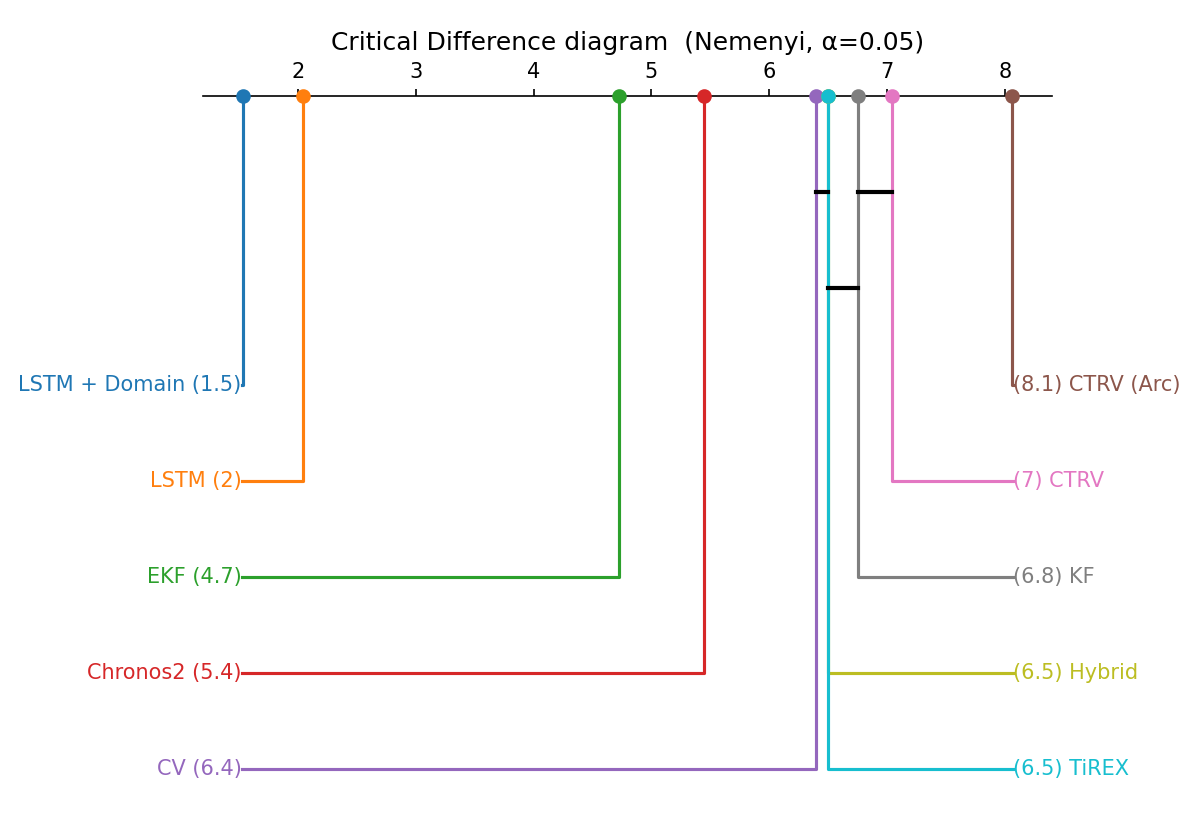
\includegraphics[width=0.7\linewidth]{figures/cd_diagram.png}
    \caption[Exp. I Friedman \& Nemenyi CD-Plot]{ \acf{CD} diagram based on the Friedman test and Nemenyi post-hoc comparison. Models connected by a horizontal bar are not significantly different at \( \alpha = 0.05\). The shown numbers are the mean rank per model in the evaluation, 1 being the best possible result.}
    \label{fig:cd_test}
\end{figure}

Figure~\ref{fig:adepredhorizon} depicts the development of the \ac{ADE} for all models over the prediction horizon. While the error for the \ac{CV} model grows approximately linearly, the errors for CTRV and CTRV Arc diverge heavily at longer horizons. The \ac{LSTM}-based models maintain the lowest \ac{ADE} across all ten prediction steps. The ranking order of all models stays consistent over the full horizon.

\begin{figure}[h]
    \centering
    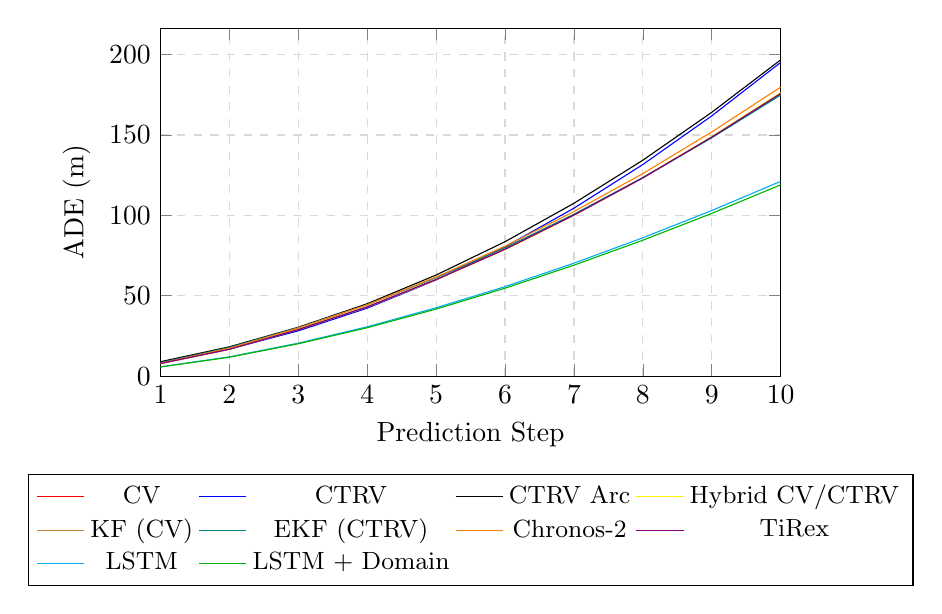
\begin{tikzpicture}
    \begin{axis}[
        width=0.78\linewidth,
        height=6cm,
        xlabel={Prediction Step},
        ylabel={ADE (m)},
        xmin=1, xmax=10,
        xtick={1,2,...,10},
        ymin=0,
        grid=major,
        grid style={dashed, gray!30},
        legend style={
            at={(0.5,-0.28)},
            anchor=north,
            legend columns=4,
            font=\small
        },
        mark size=1.5pt,
        cycle list name=color list,
    ]
    
    \addplot coordinates {
        (1,7.861)(2,16.747)(3,28.983)(4,43.096)(5,60.103)
        (6,78.936)(7,100.214)(8,123.386)(9,148.728)(10,175.824)
    }; \addlegendentry{CV}
    
    \addplot coordinates {
        (1,8.353)(2,16.865)(3,28.177)(4,42.303)(5,59.811)
        (6,80.468)(7,104.477)(8,131.658)(9,161.924)(10,195.180)
    }; \addlegendentry{CTRV}
    
    \addplot coordinates {
        (1,8.976)(2,18.242)(3,30.422)(4,45.051)(5,62.918)
        (6,83.636)(7,107.548)(8,134.347)(9,164.148)(10,196.783)
    }; \addlegendentry{CTRV Arc}
    
    \addplot coordinates {
        (1,8.054)(2,16.930)(3,29.044)(4,43.019)(5,59.942)
        (6,78.772)(7,100.143)(8,123.486)(9,149.066)(10,176.446)
    }; \addlegendentry{Hybrid CV/CTRV}
    
    \addplot coordinates {
        (1,7.861)(2,16.747)(3,28.983)(4,43.096)(5,60.103)
        (6,78.936)(7,100.216)(8,123.386)(9,148.726)(10,175.824)
    }; \addlegendentry{KF (CV)}
    
    \addplot coordinates {
        (1,8.364)(2,17.853)(3,30.191)(4,44.472)(5,61.235)
        (6,79.889)(7,100.747)(8,123.511)(9,148.295)(10,174.882)
    }; \addlegendentry{EKF (CTRV)}
    
    \addplot coordinates {
        (1,8.020)(2,17.405)(3,29.932)(4,44.419)(5,61.698)
        (6,80.865)(7,102.417)(8,126.026)(9,151.936)(10,179.800)
    }; \addlegendentry{Chronos-2}
    
    \addplot coordinates {
        (1,7.860)(2,16.743)(3,28.975)(4,43.083)(5,60.084)
        (6,78.911)(7,100.189)(8,123.362)(9,148.711)(10,175.820)
    }; \addlegendentry{TiRex}
    
    \addplot coordinates {
        (1,5.769)(2,12.005)(3,20.515)(4,30.700)(5,42.527)
        (6,55.682)(7,70.279)(8,86.083)(9,103.057)(10,121.181)
    }; \addlegendentry{LSTM}

    \addplot coordinates {
        (1,5.686)(2,11.776)(3,20.143)(4,30.110)(5,41.737)
        (6,54.729)(7,69.035)(8,84.572)(9,101.244)(10,119.017)
    }; \addlegendentry{LSTM + Domain}
    
    \end{axis}
    \end{tikzpicture}
    %\caption{ADE per prediction step averaged across all tracks 
    \caption[Exp. I ADE over Time]{Progression of \acf{ADE} over time, showing the divergence of error across all ten prediction steps. The plot demonstrates that \acf{LSTM}-based architectures achieve the lowest errors, while kinematic models exhibit higher trajectory divergence, particularly as the prediction horizon increases.}
    \label{fig:adepredhorizon}
\end{figure} 

Regarding the foundation models, Table~\ref{tab:results_exp0_foundation_prob} shows the probabilistic calibration metrics.
TiRex produces extremely narrow prediction intervals (Mean Interval Width of 6.41) and achieves a coverage of only 0.059. In contrast, Chronos-2 produces wider intervals (Mean Interval Width of 145.37) but achieves a near-ideal coverage of 0.769. %\me{move calibration to discussion?}
Figure~\ref{fig:violince} visualises the error distribution shapes as violin plots, showing that TiRex and the \ac{CV} model share nearly identical error distributions, while the \ac{LSTM} distribution is distinctly shifted toward lower errors.

Furthermore, an evaluation of the error distributions for the kinematic baselines (\ac{CV} and \ac{CTRV}) reveals a stark deviation from a normal distribution, with coefficients of determination ($R^2$) ranging from 0.6138 to 0.6428.

\begin{table}[t]
\centering
\caption{Exp. I Probabilistic metrics for foundation models}
\label{tab:results_exp0_foundation_prob}
\begin{tabular}{lrrr}
\toprule
\textbf{Model} & \textbf{MIW} & \textbf{Coverage} & \textbf{Winkler80} \\
\midrule
Chronos-2 (zero-shot) & 145.37 & 0.769 & 114.65 \\
TiRex                 &   6.41 & 0.059 & 112.20 \\
\bottomrule
\end{tabular}
\end{table}

\begin{figure}[h]
    \centering
    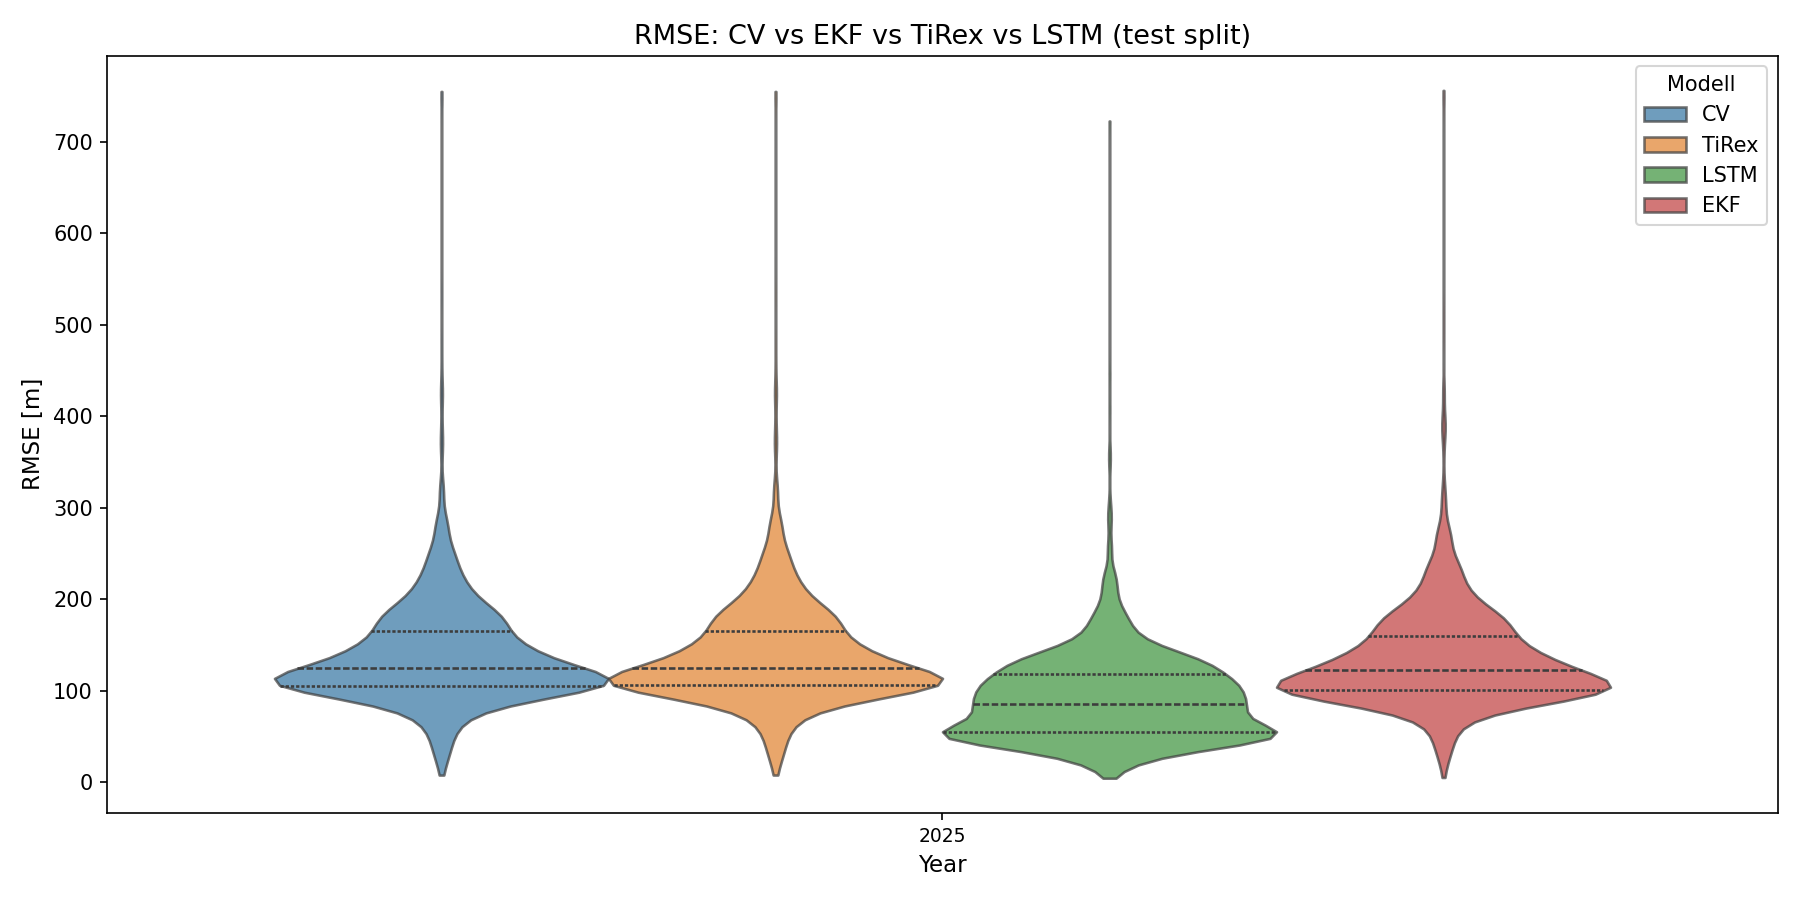
\includegraphics[width=0.98\linewidth]{test_violin_cv_ekf_tirex_lstm_per_year.png}
    %\caption{Violin Plots for CV, EKF, TiRex and LSTM}
    \caption[Exp. I RMSE Violin Plots]{Violin plots visualising the distribution of \acf{RMSE} for the \acf{CV}, \acf{EKF}, TiRex, and \acf{LSTM} models on the test set. The \ac{LSTM} model demonstrates a distinct shift toward lower error values compared to the other models, whereas the \acf{CV} and TiRex models exhibit nearly identical error distributions.}
    \label{fig:violince}
\end{figure}

Finally, the hyperparameter optimisation process for the \ac{LSTM} is visualised in % Figure ~\ref{fig:succhalfing} and
Figure~\ref{fig:paralelcord}. 
% Figure~\ref{fig:succhalfing} illustrates a successive halving run, demonstrating how underperforming configurations were pruned early.
%Figure~\ref{fig:paralelcord} 
It presents a parallel coordinate plot of the parameter search with a clear band around the optimal configuration. The plot indicates that the optimisation selected a feature set that explicitly excluded the \ac{ROT}.
Furthermore, Figure~\ref{fig:monthlytrends-all} plots the average \ac{RMSE} per month over the full dataset, with consistent performance trends across all models.

%\begin{figure}[h]
%    \centering
%    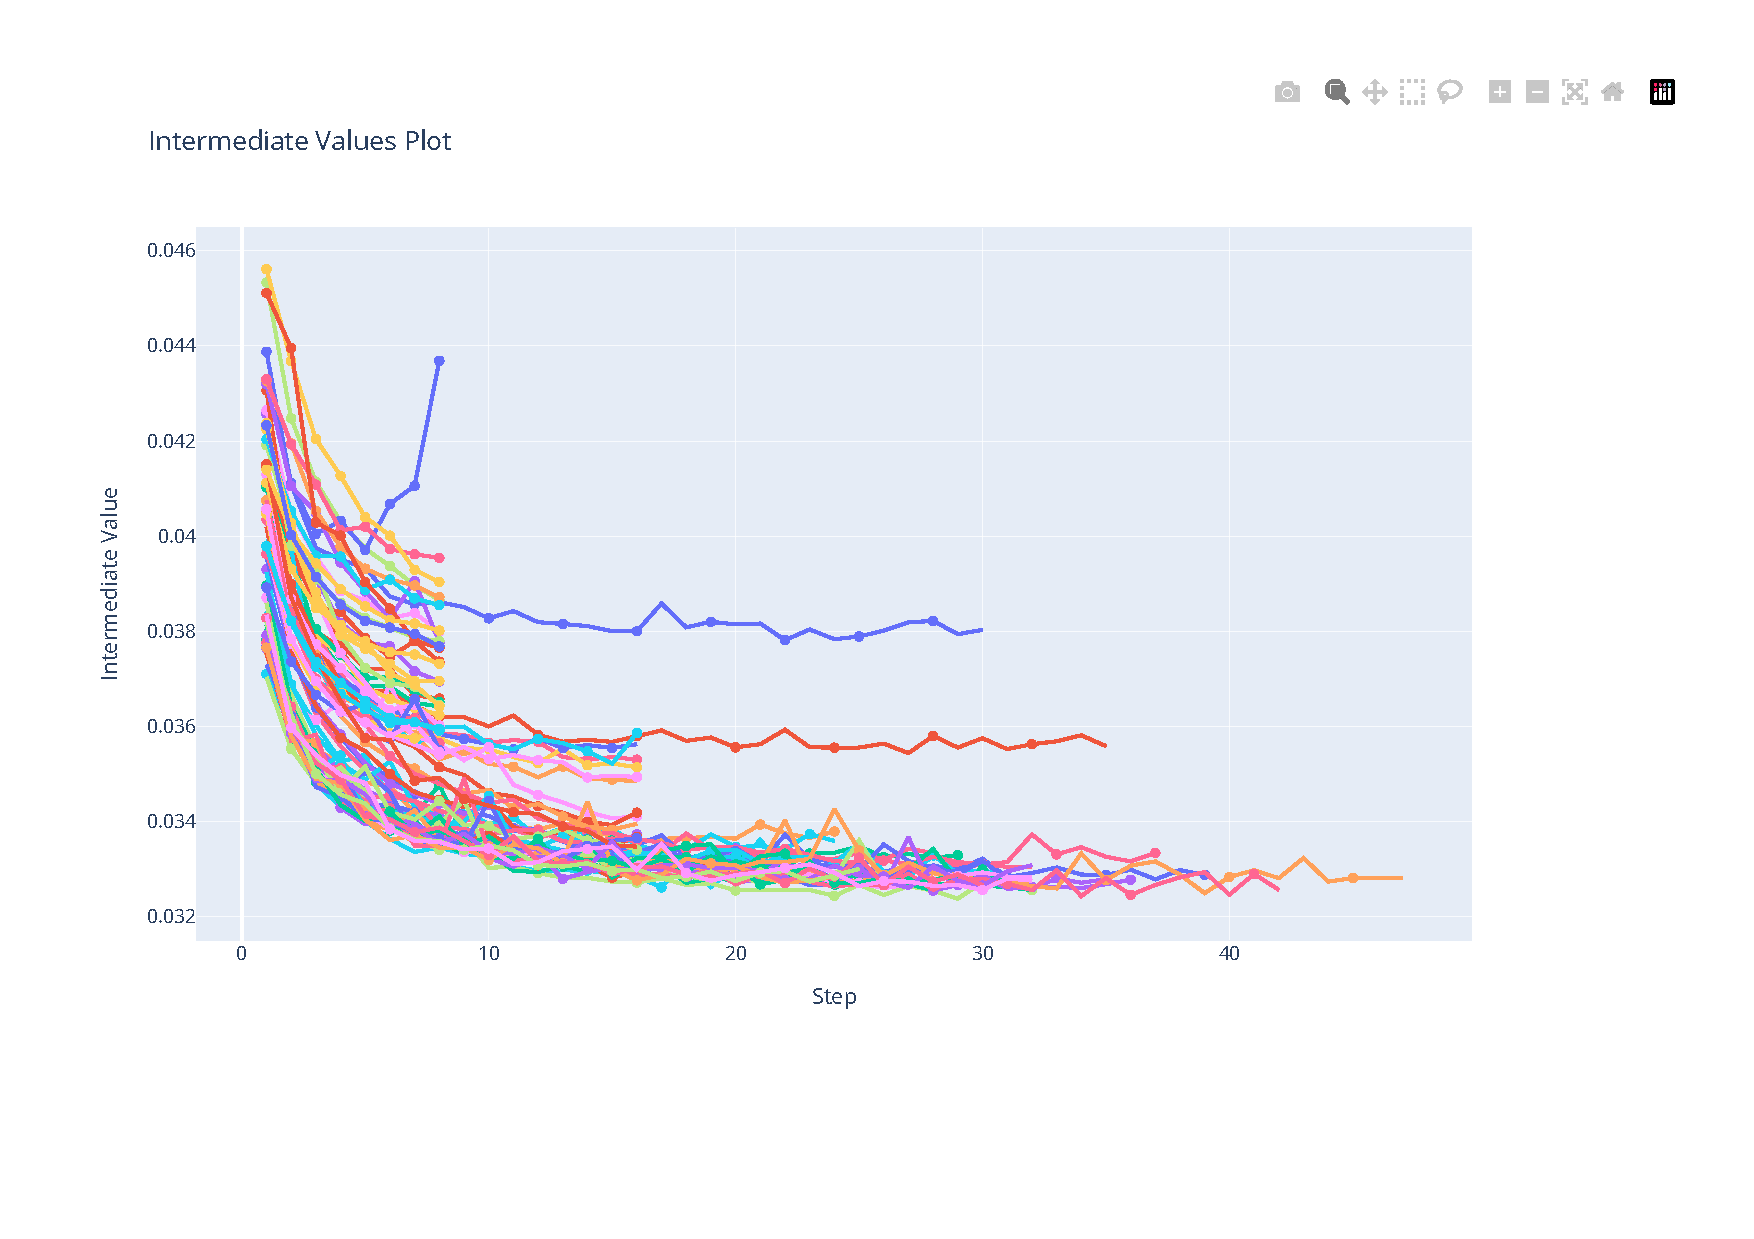
\includegraphics[width=0.9\linewidth,trim=1cm 3.5cm 5.5cm 3.5cm,clip]{figures/minimal_lstm_intermediate_values.html.pdf}
%    \caption[Exp. I LSTM Intermediate Value plot]{Intermediate Value plot of \acf{LSTM} \acf{HPO} in Optuna with early stopping enabled. Successive Halving was applied to all trials, except the initial 16. \me{should this be moved into methods, appendix? removed? it is not discussed in detail} \todo{remove all result references to this}}
%    \label{fig:succhalfing}
%\end{figure}

\begin{figure}[h]
    \centering
    %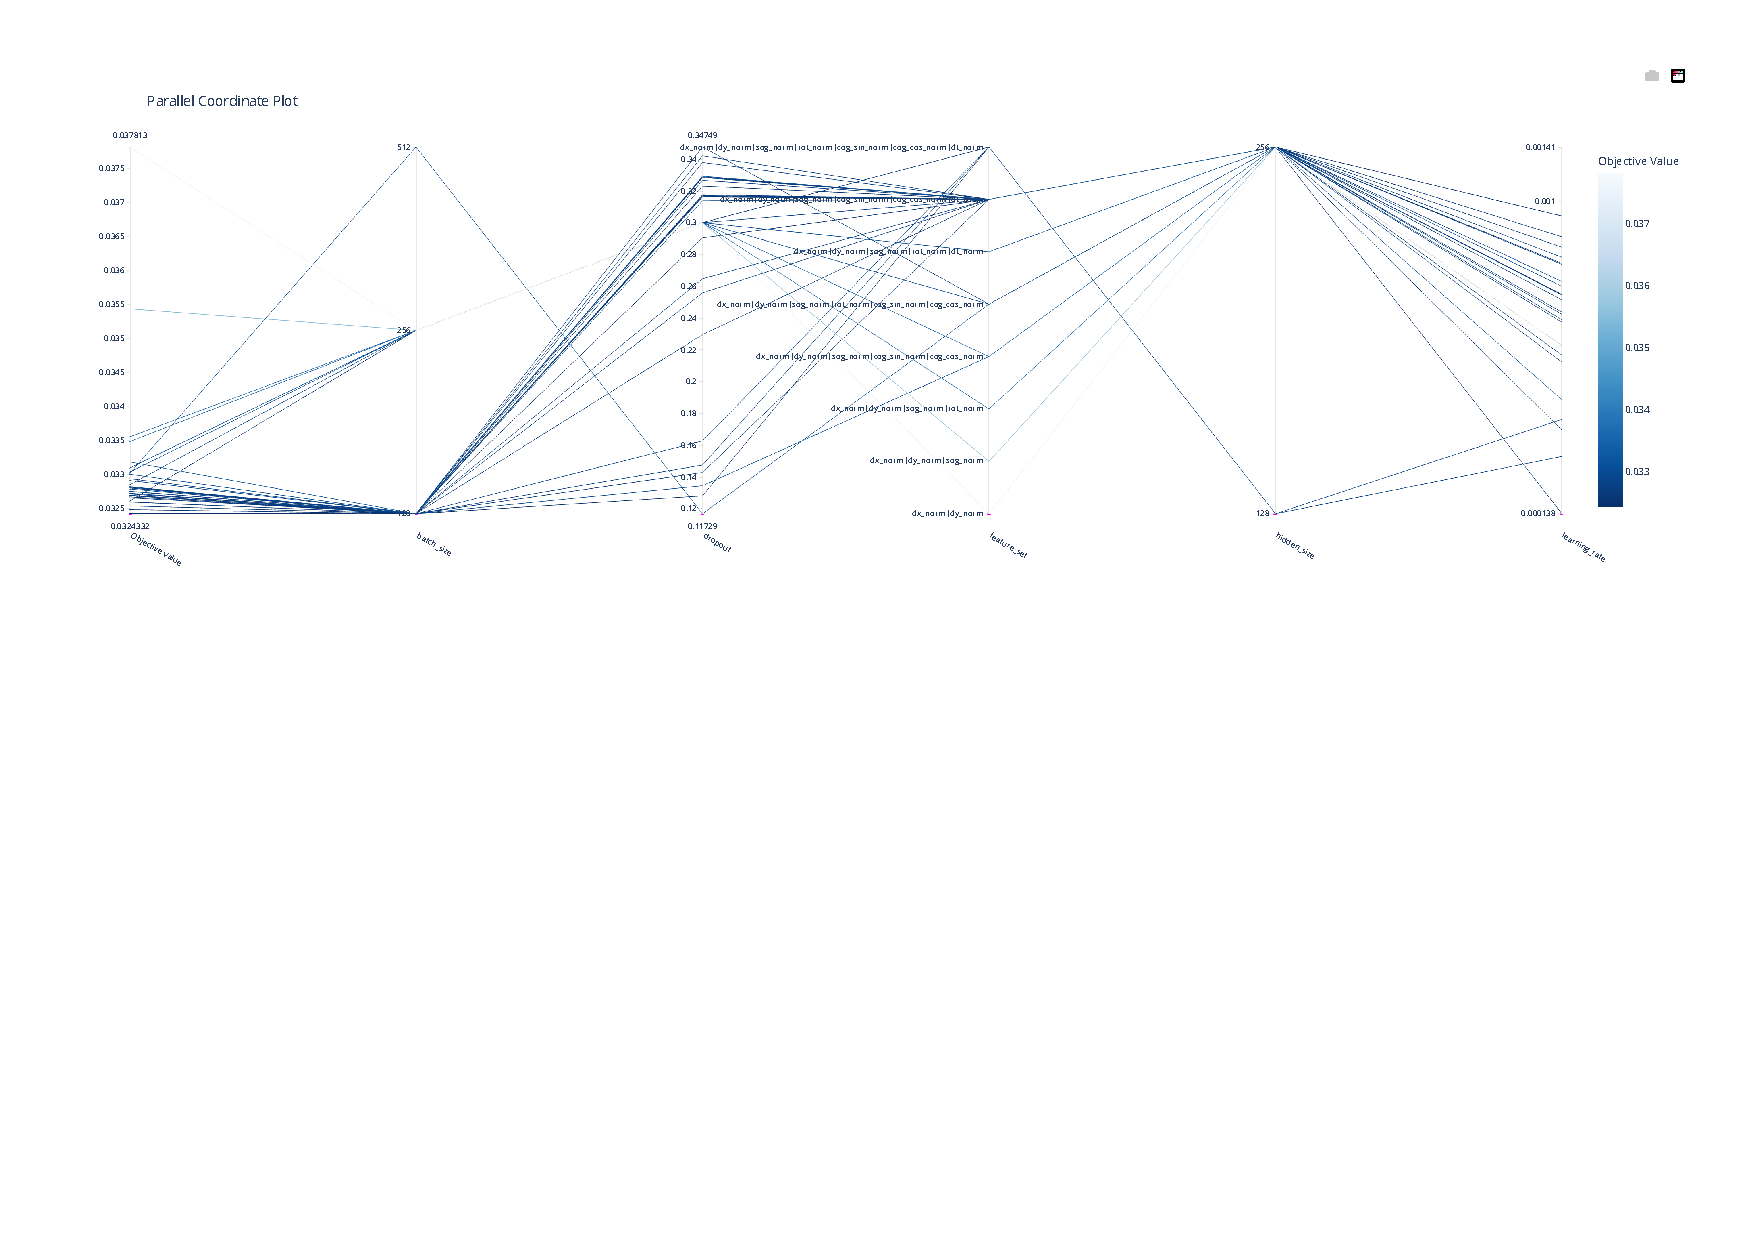
\includegraphics[width=1\linewidth,trim=1cm 10.5cm 1cm 1.5cm,clip]{figures/minimal_lstm_parallel_coordinate.html.pdf}
    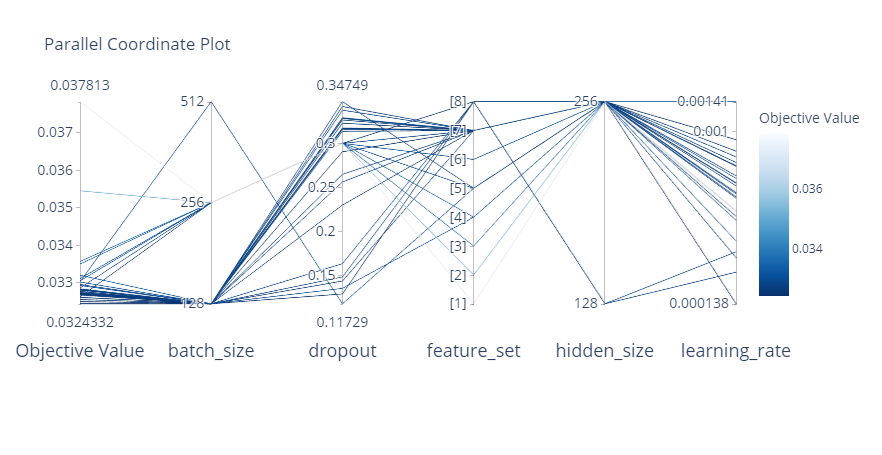
\includegraphics[width=1\linewidth, trim=0cm 3.1cm 0cm 2cm,clip]{figures/paralelcoord_zoomed.png}
    %\caption[Exp. I LSTM Parallel Coordinate Plot]{Parallel Coordinate Plot of \acf{LSTM} Hyperparameter selection, showing a clear band around the selected hyperparameter configuration. \todo{add 1, 2, 3...}}
    \caption[Exp. I LSTM Parallel Coordinate Plot]{Parallel Coordinate Plot of \acf{LSTM} Hyperparameter selection, showing a clear band around the selected hyperparameter configuration. Feature set mappings: [1] dx\_norm, dy\_norm; [2] dx\_norm, dy\_norm, sog\_norm; [3] dx\_norm, dy\_norm, sog\_norm, rot\_norm; [4] dx\_norm, dy\_norm, sog\_norm, cog\_sin\_norm, cog\_cos\_norm; [5] dx\_norm, dy\_norm, sog\_norm, rot\_norm, cog\_sin\_norm, cog\_cos\_norm; [6] dx\_norm, dy\_norm, sog\_norm, rot\_norm, dt\_norm; [7] dx\_norm, dy\_norm, sog\_norm, cog\_sin\_norm, cog\_cos\_norm, dt\_norm; [8] dx\_norm, dy\_norm, sog\_norm, rot\_norm, cog\_sin\_norm, cog\_cos\_norm, dt\_norm.} \me{new version with increased font sizes and feature sets not witten explcicitly because of overlap. now the caption is very long though, any ideas?}
    \label{fig:paralelcord}
\end{figure}


\begin{figure}[h]
    \centering
    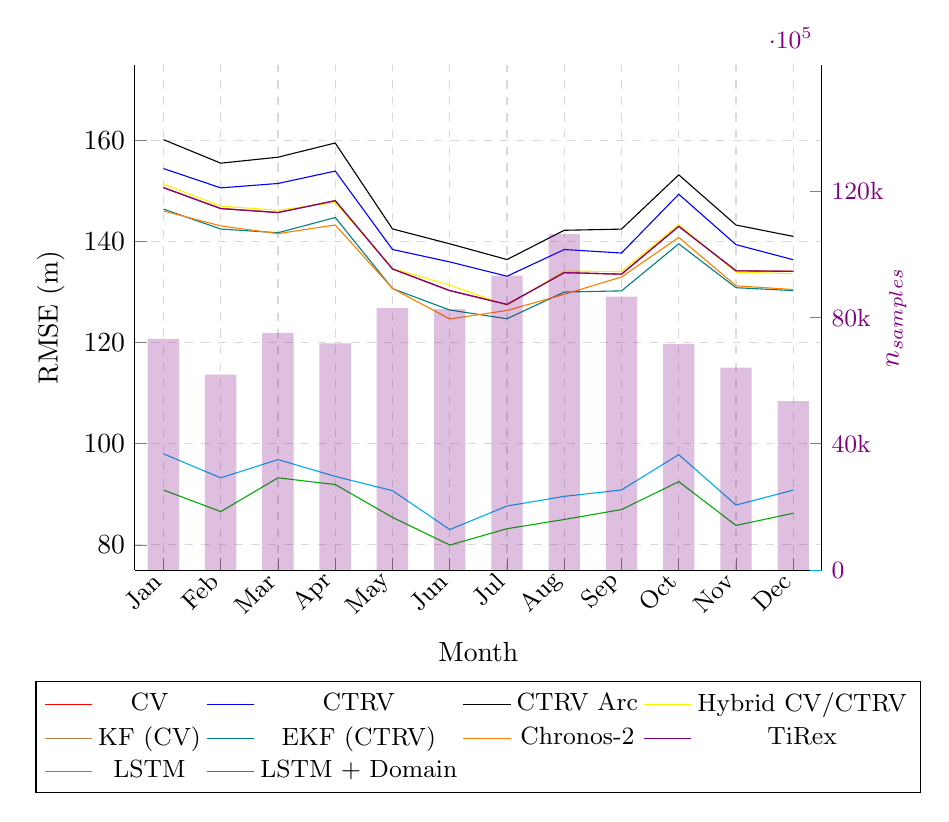
\begin{tikzpicture}
    \begin{axis}[
        name=main,
        width=0.85\linewidth,
        height=8cm, 
        xlabel={Month},
        ylabel={RMSE (m)},
        ymin=75, ymax=175, 
        xmin=0.5, xmax=12.5,
        xtick={1,2,...,12},
        xticklabels={Jan,Feb,Mar,Apr,May,Jun,Jul,Aug,Sep,Oct,Nov,Dec},
        xticklabel style={rotate=45, anchor=east, font=\small},
        grid=major,
        grid style={dashed, gray!30},
        legend style={
            at={(0.5,-0.22)},
            %at={(0.5, 1.1)},
            anchor=north,
            legend columns=4,
            font=\small
        },
        mark size=1.5pt,
        cycle list name=color list,
        axis y line*=left,
        axis x line*=bottom,
    ]
    
    \addplot coordinates {
        (1,150.68)(2,146.54)(3,145.76)(4,148.09)(5,134.58)
        (6,130.30)(7,127.56)(8,133.85)(9,133.55)(10,143.01)
        (11,134.22)(12,134.11)
    }; \addlegendentry{CV}
    
    \addplot coordinates {
        (1,154.44)(2,150.62)(3,151.49)(4,153.95)(5,138.43)
        (6,135.97)(7,133.14)(8,138.42)(9,137.73)(10,149.36)
        (11,139.39)(12,136.40)
    }; \addlegendentry{CTRV}
    
    \addplot coordinates {
        (1,160.16)(2,155.51)(3,156.69)(4,159.50)(5,142.50)
        (6,139.55)(7,136.44)(8,142.23)(9,142.46)(10,153.20)
        (11,143.27)(12,141.02)
    }; \addlegendentry{CTRV Arc}
    
    \addplot coordinates {
        (1,151.39)(2,147.01)(3,146.20)(4,147.73)(5,134.67)
        (6,131.39)(7,127.38)(8,134.15)(9,134.07)(10,143.37)
        (11,133.93)(12,133.65)
    }; \addlegendentry{Hybrid CV/CTRV}
    
    \addplot coordinates {
        (1,150.68)(2,146.54)(3,145.76)(4,148.09)(5,134.58)
        (6,130.30)(7,127.56)(8,133.85)(9,133.55)(10,143.01)
        (11,134.22)(12,134.11)
    }; \addlegendentry{KF (CV)}
    
    \addplot coordinates {
        (1,146.42)(2,142.48)(3,141.74)(4,144.76)(5,130.69)
        (6,126.45)(7,124.73)(8,130.01)(9,130.24)(10,139.55)
        (11,130.87)(12,130.29)
    }; \addlegendentry{EKF (CTRV)}
    
    \addplot coordinates {
        (1,146.06)(2,143.09)(3,141.57)(4,143.28)(5,130.72)
        (6,124.68)(7,126.37)(8,129.56)(9,132.99)(10,140.82)
        (11,131.24)(12,130.51)
    }; \addlegendentry{Chronos-2}
    
    \addplot coordinates {
        (1,150.65)(2,146.52)(3,145.73)(4,148.08)(5,134.58)
        (6,130.29)(7,127.55)(8,133.85)(9,133.54)(10,143.00)
        (11,134.21)(12,134.09)
    }; \addlegendentry{TiRex}
    
    \addplot coordinates {
        (1,98.00)(2,93.24)(3,96.86)(4,93.53)(5,90.71)
        (6,83.01)(7,87.67)(8,89.58)(9,90.85)(10,97.84)
        (11,87.86)(12,90.82)
    }; \addlegendentry{LSTM}

    \addplot coordinates {
        (1,90.84)(2,86.57)(3,93.25)(4,91.92)(5,85.43)
        (6,79.95)(7,83.18)(8,85.01)(9,86.97)(10,92.49)
        (11,83.83)(12,86.24)
    }; \addlegendentry{LSTM + Domain}
    
    \end{axis}
    
    \begin{axis}[
        width=0.85\linewidth,
        height=8cm,
        ymin=0, ymax=160000,
        xmin=0.5, xmax=12.5,
        xtick=\empty,
        ylabel={$n_\text{samples}$},
        ylabel style={at={(1.08,0.5)}, color=violet},
        ytick={0,40000,80000,120000},
        yticklabels={0,40k,80k,120k},
        yticklabel style={font=\small, color=violet},
        ytick style={color=cyan},
        axis y line*=right,
        axis x line=none,
        bar width=0.55,
    ]
    
    \addplot[ybar, fill=violet, draw=none, fill opacity=0.25] coordinates {
        (1,73177)(2,61903)(3,75120)(4,71784)(5,83023)
        (6,82636)(7,93205)(8,106326)(9,86547)(10,71582)
        (11,64072)(12,53443)
    };
    
    \end{axis}
    \end{tikzpicture}
    %\caption{RMSE per month with track count shown as violet bars\todo{from here on, expand figure and table captions}}
    \caption[Exp. I RMSE Monthly Trends]{Comparison of \acf{RMSE} by month, demonstrating consistent performance trends across all models. Violet bars indicate the monthly volume of samples}
    \label{fig:monthlytrends-all}
\end{figure}



%\section[Exp. \Romannum{2}: Domain-specific training]{Exp. \Romannum{2}: Effect of Domain-Specific Training on Predictive Performance}

%This experiment is designed to answer 
\FloatBarrier
\textbf{RQ 2}: \textit{Does domain-specific training improve short-term vessel trajectory prediction performance compared to mixed-domain training?}

We set up Exp. \Romannum{2} to evaluate the extent of these performance differences and how they are influenced by both the specific waterway domain and the underlying model complexity. %To that end, we set up Exp. \Romannum{2}.
\paragraph{Results.}

%performance between training modes
%The benefit of per-domain training increases with model complexity. %not purely descriptive
For the \ac{CV} model, no change in performance ($0.00$\,m difference) is observed between mixed and domain-specific training. Since the \ac{CV} search space consists of the single hyperparameter $n_\text{vel}$, and the optimiser converged to $n_\text{vel}=1$ in every domain as well as in the mixed setting, the resulting models are identical across all training regimes. The \ac{CTRV} variants exhibit deviations of up to $12.55$\,m in \ac{RMSE}. 
For the \ac{EKF} and \ac{LSTM}, however, substantial performance drops occur under mixed training, particularly in the channel and lock domains (Table \ref{tab:results_exp1_exp2_merged_deltas}, shaded in orange).
 Specifically, in the lock domain, the \ac{ADE} of the \ac{LSTM} degrades by $13.36$\,m and the \ac{RMSE} by $13.11$\,m when evaluated with the mixed training model.
This performance difference is not uniform across domains: in the harbour and river domains, only minor deviations are observed, generally remaining below a $5.6$\,m difference in \ac{RMSE}.
Finally, it can be observed that the harbour domain is the only environment where domain-specific training fails to produce a statistically significant improvement for the \ac{LSTM}. Further details about the statistical significance across domains can be found in Figure \ref{fig:cd-diagrams-a} in Appendix \ref{chap:appendixdataplots}.


%performance between domains
In Table~\ref{tab:results_exp1_exp2_merged_deltas}, the corresponding test set error metrics evaluated per domain are presented on the left, alongside the performance delta when evaluating the mixed training model on the right. Positive deltas indicate better performance for the models optimised on domain-specific data.
The lowest absolute errors are achieved in the channel domain; notably, the \ac{LSTM} attains an \ac{ADE} of $32.09$\,m and an \ac{RMSE} of $55.85$\,m (shaded in cyan).
Conversely, the highest errors are consistently produced in the harbour domain (e.g., an \ac{LSTM} \ac{ADE} of $61.07$\,m), making it comparatively difficult to predict.
When comparing model families, the largest relative improvements are observed in the lock and channel domains when moving from kinematic models to learned models. Changes in the harbour domain are inconsistent, with only minor improvements for the \ac{LSTM} and measurable degradation for the \ac{EKF} (a delta of $-1.47$\,m \ac{RMSE}).

%hyperparameters
In Table~\ref{tab:hpo_results_merged}, the optimised hyperparameter configurations for both mixed and domain-specific training setups are listed.
Notably, the optimised hyperparameters vary substantially across the domains.
This applies not only to the learned models but also to the Kalman filters. The optimised values for measurement noise, process noise, and initial covariance differ considerably. 
The measurement noise $r_\text{pos}$ covers nearly five orders of magnitude across models and domains, ranging from approximately $1.0\times10^{-2}$ to $7.3\times10^{2}$.
In particular, highly distinct parameter selections are yielded by the lock class for all models.
For example, very distinct hyperparameters can be observed for the \ac{LSTM} (such as a reduced hidden size of $64$ and an increased batch size of $512$). The \ac{EKF} applied to this domain is assigned a larger measurement noise $r_\text{pos}$ coupled with a very small process noise $q_\text{pos}$ (both shaded in green). 
Similarly, for TiRex and \ac{EKF}, a longer context length is selected specifically for the channel domain ($n_\text{ctx} = 9$ and $6$, respectively), while for kinematic baselines, the context length is reduced (shaded in cyan). %these are not discussed further, focus is on "yes there is a difference and it impacts performance" and not on "these are the differences and here is what it tells us about the data. in general, lots more can be discussed about specific parameters . eg how higher context windows act as a smoothness factor etc. but if we wanted to do that, we wouldnt have hpoed everything automatically
For the lock domain, in contrast, the \ac{EKF}'s context length is reduced to $n_\text{ctx}=1$. With only a single observation available before prediction begins, the filter has little opportunity to correct its $\omega_0=0$ initialisation if the vessel is already turning. Combined with the low process noise $q_\text{pos}$ and high measurement noise $r_\text{pos}$ discussed above, the filter is effectively optimised to trust its motion assumption over new measurements, which likely contributes to the disproportionately large performance gap between the \ac{EKF} and the \ac{LSTM} specifically in this domain.

\begin{comment}
\begin{table}[t]
\centering
\caption[Exp. II Optimised Hyperparameter Configurations]{Optimised hyperparameter configurations for per-domain training and mixed training. Discussed parameters are shaded in.}
\label{tab:hpo_results_merged}
\small
\setlength{\tabcolsep}{3pt}
\begin{tabular}{llrrrrr}
\toprule
\textbf{Model} & \textbf{Hyperparameter} & \textbf{Mixed} & \textbf{Harbour} & \textbf{River} & \textbf{Channel} & \textbf{Lock} \\
\midrule
CV             & $n_\text{vel}$        & 1      & 1     & 1     & 1     & 1     \\
CTRV           & $n_\text{vel}$        & 2      & 2     & 2     & \cellcolor{cyan!15}1     & 1     \\
CTRV Arc       & $n_\text{vel}$        & 3      & 3     & 3     & \cellcolor{cyan!15}2     & 1     \\
Hybrid CV/CTRV & $n_\text{vel}$ (CV)   & 1      & 1     & 1     & 1     & 1     \\
               & $n_\text{vel}$ (CTRV) & 2      & 2     & 2     & \cellcolor{cyan!15}1     & \cellcolor{orange!15}9     \\
               & $n_\text{rot}$        & 1      & 1     & 1     & 1     & \cellcolor{orange!15}9     \\
               & $\tau_\text{rot}$     & 29.28  & 29.28 & 29.28 & 1.00  & \cellcolor{orange!15}72.76 \\
\midrule
KF (CV)        & $q_\text{pos}$        & $1.578 \times 10^{-3}$ & $1.578 \times 10^{-3}$ & $2.434 \times 10^{-3}$ & $2.483 \times 10^{-3}$ & $1.578 \times 10^{-3}$ \\
               & $q_\text{vel}$        & $5.932$                & $5.932$                & $5.115$                & $9.930$                & $5.932$                \\
               & $r_\text{pos}$        & $1.077 \times 10^{-2}$ & $1.077 \times 10^{-2}$ & $3.035 \times 10^{1}$  & $1.005 \times 10^{-2}$ & $1.077 \times 10^{-2}$ \\
               & $p_{0,\text{pos}}$    & $7.737 \times 10^{-2}$ & $7.737 \times 10^{-2}$ & $2.941$                & $1.637 \times 10^{-2}$ & $7.737 \times 10^{-2}$ \\
               & $p_{0,\text{vel}}$    & $1.190 \times 10^{-1}$ & $1.190 \times 10^{-1}$ & $1.556 \times 10^{-3}$ & $3.510 \times 10^{-1}$ & $1.190 \times 10^{-1}$ \\
EKF (CTRV)     & $q_\text{pos}$        & $15.957$               & $2.067 \times 10^{-2}$ & $2.645 \times 10^{1}$  & $1.140 \times 10^{-1}$ & \cellcolor{green!15}$5.667 \times 10^{-2}$ \\
               & $q_\text{vel}$        & $4.290 \times 10^{-2}$ & $3.573 \times 10^{-1}$ & $1.646 \times 10^{-3}$ & $2.197 \times 10^{-1}$ & $3.625 \times 10^{-1}$ \\
               & $q_\text{rot}$        & $1.002 \times 10^{-7}$ & $2.206 \times 10^{-5}$ & $1.378$                & $1.295 \times 10^{-6}$ & $6.197 \times 10^{-7}$ \\
               & $r_\text{pos}$        & $1.792 \times 10^{-2}$ & $4.662 \times 10^{-2}$ & $9.167 \times 10^{-1}$ & $2.378 \times 10^{1}$  & \cellcolor{green!15}$7.339 \times 10^{2}$  \\
               & $p_{0,\text{pos}}$    & $4.046 \times 10^{-1}$ & $4.862 \times 10^{2}$  & $4.471 \times 10^{-1}$ & $4.161 \times 10^{2}$  & $2.951 \times 10^{3}$  \\
               & $p_{0,\text{vel}}$    & $1.845 \times 10^{-3}$ & $1.713 \times 10^{-2}$ & $3.479 \times 10^{-4}$ & $6.428 \times 10^{1}$  & $1.348 \times 10^{-4}$ \\
               & $p_{0,\text{rot}}$    & $2.076 \times 10^{-6}$ & $3.404 \times 10^{-1}$ & $1.896 \times 10^{-6}$ & $3.569 \times 10^{-6}$ & $7.577 \times 10^{-5}$ \\
               & $n_\text{ctx}$        & 2                      & 1                      & 1                      & \cellcolor{cyan!15}6   & 1                      \\
\midrule
Chronos-2      & \textit{no HPO}        & --     & --     & --     & --     & --    \\
TiRex          & context length        & 1      & 1      & 1      & \cellcolor{cyan!15}9      & 1     \\
\midrule
LSTM           & hidden size           & 256   & 256   & 256   & 128   & \cellcolor{orange!15}64   \\
               %& num.\ layers          & 2     & --    & --    & --    & --    \\
               & dropout               & 0.290 & 0.232 & 0.377 & 0.165 & 0.378 \\
               & learning rate         & $5.530 \times 10^{-4}$ & $4.852 \times 10^{-4}$ & $1.935 \times 10^{-4}$ & $9.003 \times 10^{-4}$ & $3.049 \times 10^{-3}$ \\
               & batch size            & 128   & 128   & 256   & 128   & \cellcolor{orange!15}512   \\
               & feature set           & no rot   & all   & all   & all   & \cellcolor{orange!15}no sog, no dt \\
\bottomrule
\end{tabular}
\end{table}

\begin{table}[t]
\centering
\caption[Exp. II Error Metrics]{Test set error metrics for mixed training and separated training, evaluated per domain. Per-domain results are represented as a delta to the mixed training results. Discussed results are shaded in.} 
\label{tab:results_exp1_exp2_merged_deltas}
\setlength{\tabcolsep}{3pt} 

\begin{tabular}{llrrrrrrrr}
\toprule
\textbf{Model} & \textbf{Metric} & 
\multicolumn{4}{c}{\textbf{Mixed Training}} & 
\multicolumn{4}{c}{\textbf{$\Delta$ (Mixed Training -- Per-domain)}} \\
\cmidrule(l){3-6} \cmidrule(l){7-10}
& & 
\textbf{Harbour} & \textbf{River} & \textbf{Channel} & \textbf{Lock} &
\textbf{Harbour} & \textbf{River} & \textbf{Channel} & \textbf{Lock} \\
\midrule
Constant Velocity   
& ADE  & 81.76 & 69.84 & 73.45 & 73.47 & 0 & 0 & 0 & 0 \\
& FDE  & 182.44 & 157.16 & 171.98 & 167.58 & 0 & 0 & 0 & 0 \\
& RMSE & 166.25 & 134.29 & 110.43 & 100.73 & 0 & 0 & 0 & 0 \\
\midrule
CTRV                
& ADE  & 89.94 & 68.47 & 62.48 & 86.55 & 0 & 0 & +0.98 & +6.23 \\
& FDE  & 212.11 & 160.64 & 145.04 & 197.34 & 0 & 0 & -1.36 & +9.93 \\
& RMSE & 178.60 & 135.47 & 96.58 & 116.72 & 0 & 0 & +0.07 & +6.10 \\
\midrule
CTRV Arc            
& ADE  & 92.44 & 69.83 & 65.58 & 94.17 & 0 & 0 & +3.33 & +12.46 \\
& FDE  & 213.77 & 160.82 & 150.38 & 210.11 & 0 & 0 & +3.27 & +20.13 \\
& RMSE & 182.62 & 138.41 & 100.85 & 125.02 & 0 & 0 & +3.16 & +12.55 \\
\midrule
Hybrid CV/CTRV      
& ADE  & 81.89 & 69.86 & 73.56 & 74.80 & 0 & 0 & +12.09 & +1.33 \\
& FDE  & 183.25 & 157.30 & 172.28 & 170.91 & 0 & 0 & +26.05 & +3.33 \\
& RMSE & 166.02 & 133.90 & 110.61 & 103.15 & 0 & 0 & +14.03 & +2.42 \\
\midrule
KF (CV)             
& ADE  & 81.76 & 69.84 & 73.45 & 73.47 & 0 & +0.13 & 0 & 0 \\
& FDE  & 182.44 & 157.16 & 171.98 & 167.58 & 0 & +0.18 & 0 & 0 \\
& RMSE & 166.25 & 134.29 & 110.43 & 100.73 & 0 & +0.02 & 0 & 0 \\
\midrule
EKF (CTRV)          
& ADE  & 82.79 & 70.84 & 68.35 & 76.53 & -1.43 & +0.50 & +6.43 & +3.06 \\
& FDE  & 182.93 & 155.95 & 158.69 & 173.23 & -1.42 & -1.56 & +13.67 & +5.65 \\
& RMSE & 162.19 & 130.09 & 103.00 & 103.89 & -1.47 & -3.46 & +7.05 & +3.16 \\
\midrule
Chronos-2           
& ADE  & 84.88 & 72.47 & 61.62 & 64.92 & 0 & 0 & 0 & 0 \\
& FDE  & 189.21 & 162.80 & 145.44 & 154.50 & 0 & 0 & 0 & 0 \\
& RMSE & 163.56 & 133.37 & 97.09 & 94.87 & 0 & 0 & 0 & 0 \\
\midrule
TiRex               
& ADE  & 81.76 & 69.78 & 73.50 & 73.47 & 0 & 0 & +4.39 & 0 \\
& FDE  & 182.44 & 157.14 & 172.00 & 167.58 & 0 & 0 & +7.21 & 0 \\
& RMSE & 166.24 & 134.22 & 110.46 & 100.73 & 0 & 0 & +3.11 & 0 \\
\midrule
LSTM                

& ADE  & 61.07 & 43.29 & \cellcolor{cyan!15}{32.09} & 45.41 & +0.39 & +3.01 & \cellcolor{orange!15}+4.81 & \cellcolor{orange!15}+13.36 \\
& FDE  & 135.73 & 94.14 & \cellcolor{cyan!15}{70.23} & 93.17 & +1.12 & +7.26 & \cellcolor{orange!15}+11.09 & \cellcolor{orange!15}+26.54 \\
& RMSE & 121.45 & 91.59 & \cellcolor{cyan!15}{55.85} & 68.59 & +0.50 & +5.51 & \cellcolor{orange!15}+7.36 & \cellcolor{orange!15}+13.11 \\
\bottomrule
\end{tabular}
\end{table}

\end{comment}

%yes this is a bit tight, but font only slightly smaller and merging them onto 1 page saves us 1 page in total, so here i am making that compromise.
\begin{table}[htbp] % h: here, t: top, b: bottom, p: page - gibt LaTeX mehr Freiheit
\centering
\vspace{-1em}%alles bischen hoch
\caption[Exp. II Optimised Hyperparameter Configurations]{Optimised hyperparameter configurations for per-domain training and mixed training. Discussed parameters are shaded in.}
\label{tab:hpo_results_merged}
\vspace{-0.3em} % Zieht die untere Tabelle näher heran (verringert Whitespace)
% \footnotesize % Noch etwas kleiner als \small, oft der Retter für große Tabellen
\fontsize{9pt}{9.5pt}\selectfont
\renewcommand{\arraystretch}{0.85} % Reduziert den Zeilenabstand (Default ist 1.0)
\setlength{\tabcolsep}{3pt}
\begin{tabular}{llrrrrr}
\toprule
\textbf{Model} & \textbf{Hyperparameter} & \textbf{Mixed} & \textbf{Harbour} & \textbf{River} & \textbf{Channel} & \textbf{Lock} \\
\midrule
CV             & $n_\text{vel}$        & 1      & 1     & 1     & 1     & 1     \\
CTRV           & $n_\text{vel}$        & 2      & 2     & 2     & \cellcolor{cyan!15}1     & 1     \\
CTRV Arc       & $n_\text{vel}$        & 3      & 3     & 3     & \cellcolor{cyan!15}2     & 1     \\
Hybrid CV/CTRV & $n_\text{vel}$ (CV)   & 1      & 1     & 1     & 1     & 1     \\
               & $n_\text{vel}$ (CTRV) & 2      & 2     & 2     & \cellcolor{cyan!15}1     & \cellcolor{orange!15}9     \\
               & $n_\text{rot}$        & 1      & 1     & 1     & 1     & \cellcolor{orange!15}9     \\
               & $\tau_\text{rot}$     & 29.28  & 29.28 & 29.28 & 1.00  & \cellcolor{orange!15}72.76 \\
\midrule
KF (CV)        & $q_\text{pos}$        & $1.578 \times 10^{-3}$ & $1.578 \times 10^{-3}$ & $2.434 \times 10^{-3}$ & $2.483 \times 10^{-3}$ & $1.578 \times 10^{-3}$ \\
               & $q_\text{vel}$        & $5.932$                & $5.932$                & $5.115$                & $9.930$                & $5.932$                \\
               & $r_\text{pos}$        & $1.077 \times 10^{-2}$ & $1.077 \times 10^{-2}$ & $3.035 \times 10^{1}$  & $1.005 \times 10^{-2}$ & $1.077 \times 10^{-2}$ \\
               & $p_{0,\text{pos}}$    & $7.737 \times 10^{-2}$ & $7.737 \times 10^{-2}$ & $2.941$                & $1.637 \times 10^{-2}$ & $7.737 \times 10^{-2}$ \\
               & $p_{0,\text{vel}}$    & $1.190 \times 10^{-1}$ & $1.190 \times 10^{-1}$ & $1.556 \times 10^{-3}$ & $3.510 \times 10^{-1}$ & $1.190 \times 10^{-1}$ \\
EKF (CTRV)     & $q_\text{pos}$        & $15.957$               & $2.067 \times 10^{-2}$ & $2.645 \times 10^{1}$  & $1.140 \times 10^{-1}$ & \cellcolor{green!15}$5.667 \times 10^{-2}$ \\
               & $q_\text{vel}$        & $4.290 \times 10^{-2}$ & $3.573 \times 10^{-1}$ & $1.646 \times 10^{-3}$ & $2.197 \times 10^{-1}$ & $3.625 \times 10^{-1}$ \\
               & $q_\text{rot}$        & $1.002 \times 10^{-7}$ & $2.206 \times 10^{-5}$ & $1.378$                & $1.295 \times 10^{-6}$ & $6.197 \times 10^{-7}$ \\
               & $r_\text{pos}$        & $1.792 \times 10^{-2}$ & $4.662 \times 10^{-2}$ & $9.167 \times 10^{-1}$ & $2.378 \times 10^{1}$  & \cellcolor{green!15}$7.339 \times 10^{2}$  \\
               & $p_{0,\text{pos}}$    & $4.046 \times 10^{-1}$ & $4.862 \times 10^{2}$  & $4.471 \times 10^{-1}$ & $4.161 \times 10^{2}$  & $2.951 \times 10^{3}$  \\
               & $p_{0,\text{vel}}$    & $1.845 \times 10^{-3}$ & $1.713 \times 10^{-2}$ & $3.479 \times 10^{-4}$ & $6.428 \times 10^{1}$  & $1.348 \times 10^{-4}$ \\
               & $p_{0,\text{rot}}$    & $2.076 \times 10^{-6}$ & $3.404 \times 10^{-1}$ & $1.896 \times 10^{-6}$ & $3.569 \times 10^{-6}$ & $7.577 \times 10^{-5}$ \\
               & $n_\text{ctx}$        & 2                      & 1                      & 1                      & \cellcolor{cyan!15}6   & 1                      \\
\midrule
TiRex          & context length        & 1      & 1      & 1      & \cellcolor{cyan!15}9      & 1     \\
\midrule
LSTM           & hidden size           & 256   & 256   & 256   & 128   & \cellcolor{orange!15}64   \\
               & dropout               & 0.290 & 0.232 & 0.377 & 0.165 & 0.378 \\
               & learning rate         & $5.530 \times 10^{-4}$ & $4.852 \times 10^{-4}$ & $1.935 \times 10^{-4}$ & $9.003 \times 10^{-4}$ & $3.049 \times 10^{-3}$ \\
               & batch size            & 128   & 128   & 256   & 128   & \cellcolor{orange!15}512   \\
               & feature set           & no rot   & all   & all   & all   & \cellcolor{orange!15}no sog, no dt \\
\bottomrule
\end{tabular}
\vspace{-0.2em} % Zieht die untere Tabelle näher heran (verringert Whitespace)
\end{table}

\begin{table}[htbp]
\centering
\caption[Exp. II Error Metrics]{Test set error metrics for mixed training and separated training, evaluated per domain. Per-domain results are represented as a delta to the mixed training results. Discussed results are shaded in.} 
\label{tab:results_exp1_exp2_merged_deltas}
\vspace{-0.3em}
%\small % Hier ebenfalls Schriftgröße anpassen
\fontsize{9pt}{9.5pt}\selectfont
\renewcommand{\arraystretch}{0.85} % Reduziert den Zeilenabstand
\setlength{\tabcolsep}{3pt} 
\begin{tabular}{llrrrrrrrr}
\toprule
\textbf{Model} & \textbf{Metric} & 
\multicolumn{4}{c}{\textbf{Mixed Training}} & 
\multicolumn{4}{c}{\textbf{$\Delta$ (Mixed Training -- Per-domain)}} \\
\cmidrule(lr){3-6} \cmidrule(l){7-10} % (lr) macht den Strich etwas hübscher (Abstand zw. Spalten)
& & 
\textbf{Harbour} & \textbf{River} & \textbf{Channel} & \textbf{Lock} &
\textbf{Harbour} & \textbf{River} & \textbf{Channel} & \textbf{Lock} \\
\midrule
Constant Velocity   
& ADE  & 81.76 & 69.84 & 73.45 & 73.47 & 0 & 0 & 0 & 0 \\
& FDE  & 182.44 & 157.16 & 171.98 & 167.58 & 0 & 0 & 0 & 0 \\
& RMSE & 166.25 & 134.29 & 110.43 & 100.73 & 0 & 0 & 0 & 0 \\
\midrule
CTRV                
& ADE  & 89.94 & 68.47 & 62.48 & 86.55 & 0 & 0 & +0.98 & +6.23 \\
& FDE  & 212.11 & 160.64 & 145.04 & 197.34 & 0 & 0 & -1.36 & +9.93 \\
& RMSE & 178.60 & 135.47 & 96.58 & 116.72 & 0 & 0 & +0.07 & +6.10 \\
\midrule
CTRV Arc            
& ADE  & 92.44 & 69.83 & 65.58 & 94.17 & 0 & 0 & +3.33 & +12.46 \\
& FDE  & 213.77 & 160.82 & 150.38 & 210.11 & 0 & 0 & +3.27 & +20.13 \\
& RMSE & 182.62 & 138.41 & 100.85 & 125.02 & 0 & 0 & +3.16 & +12.55 \\
\midrule
Hybrid CV/CTRV      
& ADE  & 81.89 & 69.86 & 73.56 & 74.80 & 0 & 0 & +12.09 & +1.33 \\
& FDE  & 183.25 & 157.30 & 172.28 & 170.91 & 0 & 0 & +26.05 & +3.33 \\
& RMSE & 166.02 & 133.90 & 110.61 & 103.15 & 0 & 0 & +14.03 & +2.42 \\
\midrule
KF (CV)             
& ADE  & 81.76 & 69.84 & 73.45 & 73.47 & 0 & +0.13 & 0 & 0 \\
& FDE  & 182.44 & 157.16 & 171.98 & 167.58 & 0 & +0.18 & 0 & 0 \\
& RMSE & 166.25 & 134.29 & 110.43 & 100.73 & 0 & +0.02 & 0 & 0 \\
\midrule
EKF (CTRV)          
& ADE  & 82.79 & 70.84 & 68.35 & 76.53 & -1.43 & +0.50 & +6.43 & +3.06 \\
& FDE  & 182.93 & 155.95 & 158.69 & 173.23 & -1.42 & -1.56 & +13.67 & +5.65 \\
& RMSE & 162.19 & 130.09 & 103.00 & 103.89 & -1.47 & -3.46 & +7.05 & +3.16 \\
\midrule
Chronos-2           
& ADE  & 84.88 & 72.47 & 61.62 & 64.92 & 0 & 0 & 0 & 0 \\
& FDE  & 189.21 & 162.80 & 145.44 & 154.50 & 0 & 0 & 0 & 0 \\
& RMSE & 163.56 & 133.37 & 97.09 & 94.87 & 0 & 0 & 0 & 0 \\
\midrule
TiRex               
& ADE  & 81.76 & 69.78 & 73.50 & 73.47 & 0 & 0 & +4.39 & 0 \\
& FDE  & 182.44 & 157.14 & 172.00 & 167.58 & 0 & 0 & +7.21 & 0 \\
& RMSE & 166.24 & 134.22 & 110.46 & 100.73 & 0 & 0 & +3.11 & 0 \\
\midrule
LSTM                

& ADE  & 61.07 & 43.29 & \cellcolor{cyan!15}{32.09} & 45.41 & +0.39 & +3.01 & \cellcolor{orange!15}+4.81 & \cellcolor{orange!15}+13.36 \\
& FDE  & 135.73 & 94.14 & \cellcolor{cyan!15}{70.23} & 93.17 & +1.12 & +7.26 & \cellcolor{orange!15}+11.09 & \cellcolor{orange!15}+26.54 \\
& RMSE & 121.45 & 91.59 & \cellcolor{cyan!15}{55.85} & 68.59 & +0.50 & +5.51 & \cellcolor{orange!15}+7.36 & \cellcolor{orange!15}+13.11 \\
\bottomrule
\end{tabular}
\end{table}

%\section[Exp. \Romannum{3}: LSTM Domain Encoding]{Exp. \Romannum{3}: Ablation of Explicit Domain Encoding for LSTMs}
\label{sec:exp3}

%This final experiment is designed to answer 
\FloatBarrier
\textbf{RQ3}: \textit{Does adding explicit domain information as one-hot encoded input improve short-term
vessel trajectory prediction performance?}
To answer this, we set up Exp. \Romannum{3}.
\paragraph{Results.}

In Table~\ref{tab:results_exp3}, we recall the performance metrics of the standard \ac{LSTM} (first introduced in Table \ref{tab:results_exp0} and \ref{tab:results_exp1_exp2_merged_deltas}) as a benchmark for comparison, alongside the metrics of two domain-aware variants: LSTM + Domain, which was independently tuned using a separate hyperparameter optimisation study, and LSTM + Domain*, a variant using the exact same hyperparameter configuration as the baseline architecture. 
Both domain-aware models achieve lower overall error metrics than the standard \ac{LSTM}. For example, the LSTM + Domain* variant reduces the overall \ac{RMSE} from $111.36$\,m to $110.20$\,m, representing a decrease of $1.04\%$.
This overall figure is dominated by the harbour domain, which accounts for the majority of samples and shows almost no improvement ($121.45$ m to $121.38$ m \ac{RMSE}), mirroring the finding from Exp.~\Romannum{2}. The channel and lock domains, by contrast, show substantially larger relative gains (shaded in cyan). For instance, the \ac{ADE} decreases from $32.09$\,m to $29.22$\,m in the channel domain, and from $45.41$\,m to $31.43$\,m in the lock domain.
To ensure that the observed performance gap is robust, the baseline \ac{LSTM} and the LSTM + Domain* model were trained ten times with different random seeds. Across all ten runs, strictly lower test errors in \acs{ADE}, \acs{FDE}, and \acs{RMSE} were recorded for the LSTM + Domain* model.
In Figure~\ref{fig:violindomaine}, the corresponding performance distributions of both models are presented.
Finally, the combined critical difference diagram confirming this statistical significance is depicted in Figure~\ref{fig:cd_exp3_real}, with the \ac{LSTM} + Domain* model ranking 1.71 on average, \ac{LSTM} + Domain achieving an average rank of 1.85 and the default \ac{LSTM} ranking last at 2.44.



\begin{table}[t]
\centering
\caption[Exp. III Error Metrics]{Test set error metrics comparing the \acs{LSTM} variants with and without Domain specific training. LSTM + Domain* refers to the LSTM + Domain model that was run using the hyperparameters of the LSTM without any optimisation. Discussed performance improvements are shaded in.}
\label{tab:results_exp3}
\begin{tabular}{llrrrrr}
\toprule
\textbf{Model} & \textbf{Metric} & \textbf{Overall} & \textbf{Harbour} & \textbf{River} & \textbf{Channel} & \textbf{Lock} \\
\midrule
LSTM            & ADE  & 54.78 & 61.07 & 43.29 & 32.09 & 45.41 \\
                & FDE  & 121.18 & 135.73 & 94.14 & 70.23 & 93.17 \\
                & RMSE & 111.36 & 121.45 & 91.59 & 55.85 & 68.59 \\
\midrule
LSTM + Domain   & ADE  & 53.80 & 60.79 & 40.79 & 29.53 & 34.94 \\
                & FDE  & 119.02 & 135.29 & 88.16 & 64.00 & 74.15 \\
                & RMSE & 109.95 & 121.01 & 86.77 & 51.07 & 55.27 \\
\midrule
LSTM + Domain* & ADE  & 53.80 & 60.70 & 41.12 & \cellcolor{cyan!15}29.22 & \cellcolor{cyan!15}31.43 \\
                & FDE  & 118.62 & 134.73 & 88.44 & \cellcolor{cyan!15}63.05 & \cellcolor{cyan!15}65.02 \\
                & RMSE & 110.20 & 121.38 & 86.72 & \cellcolor{cyan!15}50.23 & \cellcolor{cyan!15}50.77 \\
\bottomrule
\end{tabular}
\end{table}

\begin{figure}[h]
    \centering
    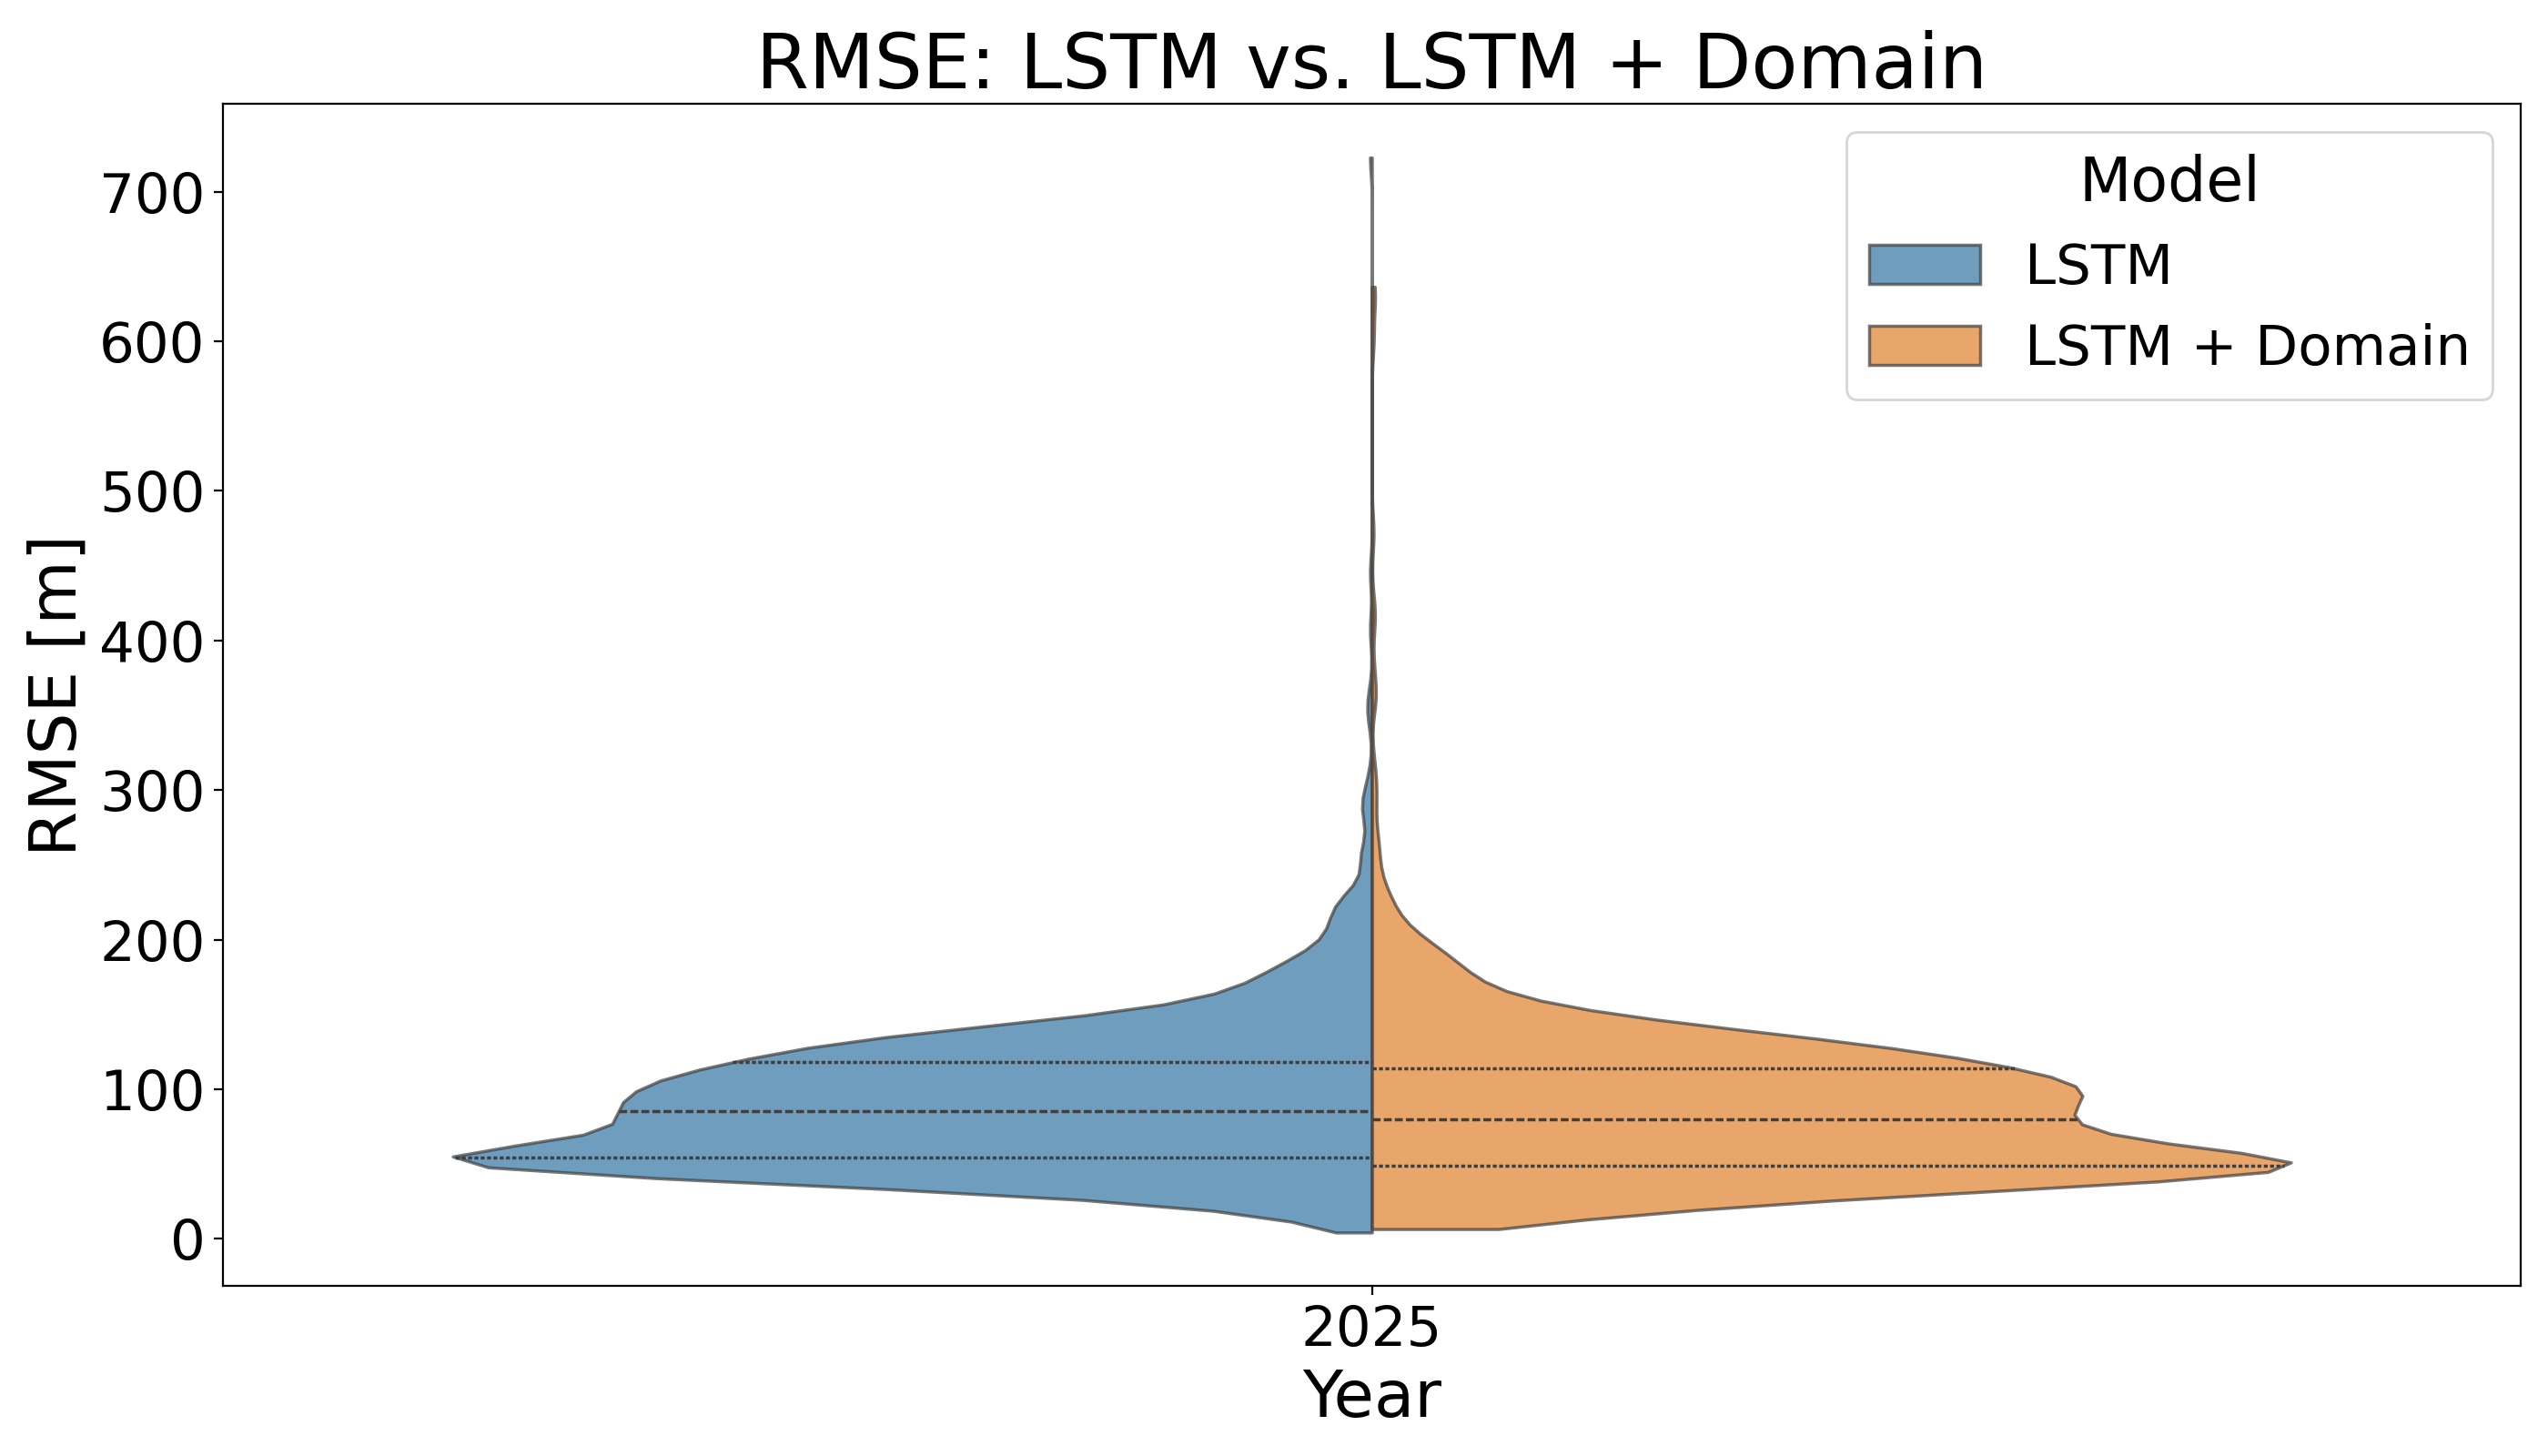
\includegraphics[width=0.7\linewidth]{figures/thesis_violin_lstm_vs_nohpo_lstm_domain_per_year.png}
    \caption[Exp. III RMSE Violin Plot]{\ac{RMSE} violin plot comparing the standard \acf{LSTM} and the \ac{LSTM} + Domain* models on the full test set.}        \label{fig:violindomaine}
\end{figure}

\begin{figure}
    \centering
    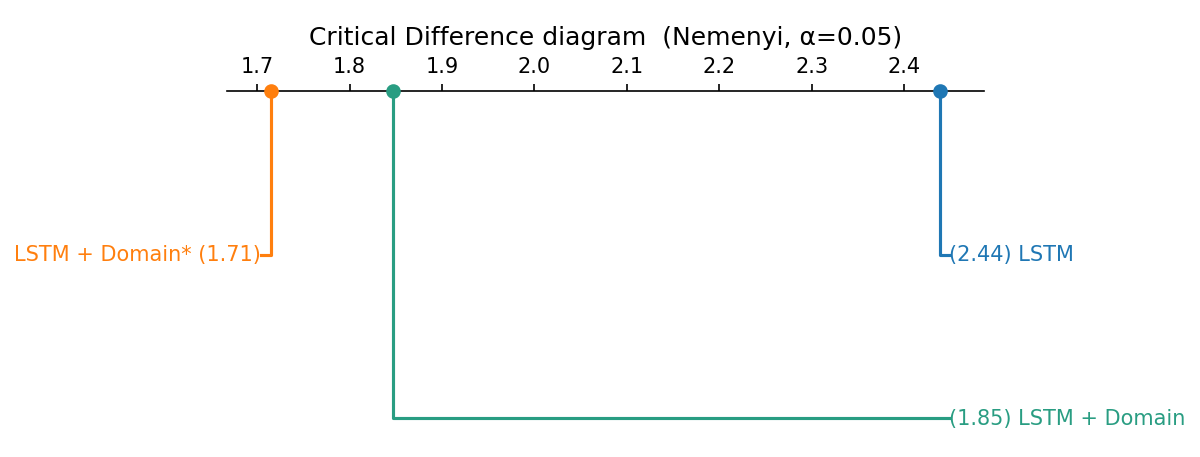
\includegraphics[width=0.7\linewidth]{figures/cd_diagram_lstm_comparison.png}
    \caption[Exp. III Friedman \& Nemenyi CD-Plot]{Critical Difference diagram comparing the \acf{LSTM} variants with and without Domain specific training.
\ac{LSTM} +Domain* refers to the \ac{LSTM} + Domain model that was run using the hyperparameters of the \ac{LSTM}
without any optimisation.}
    \label{fig:cd_exp3_real}
\end{figure}


\section*{Further Analysis}%titel anpassen


%In the preceding sections, we have shown the quantitative outcomes for each research question. 
In what follows, we discuss the mechanisms and implications behind these results, starting with a comparison of predictive capabilities across all evaluated model families, followed by an investigation of the impact of geographic domains and their encodings to model performance, and ending with a brief section on monthly trends.   

\subsection*{Predictive Capabilities of Motion Models} %was comparing. could be comparison of, but needs to be action


%\subsection{Exp. 1 Discussion}

The results provide a clear answer to the first research question: learned sequence models, particularly task-specific \acp{LSTM}, significantly outperform both classical kinematic models and stochastic filters in predicting short-term inland vessel trajectories. Following, we investigate each model family in more detail.

\paragraph{Kinematic Models.}
The performance of the kinematic models suggests that simple arc estimations are insufficient to outperform straight-line motion prediction. The \ac{CV} model learned to only use the velocity of the most recent timestep (highlighted in purple in Table~\ref{tab:hpo_results_exp0}).
This is an assumption that is also applied in most \ac{CV} definitions, which was relaxed for these experiments by parametrising context length. 
An analysis of the error distributions for the \ac{CV} and \ac{CTRV} models reveals that the resulting residuals are heavy-tailed rather than normally distributed. This deviation is reflected by low coefficient of determination ($R^2$) values of approximately 0.6138 to 0.6428 when compared against a theoretical normal distribution. Further analysis of this error distribution can be found in Figure \ref{fig:qqplot} in Appendix~\ref{chap:appendixdataplots}.
This observation leads us to a likely explanation for the optimisation result: vessel displacement over our samples could be dominated by brief, discrete regime changes rather than smooth, Gaussian drift. Averaging the displacement would therefore mix in an increasingly stale velocity estimate rather than reduce noise, so the most recent single step remains the least biased predictor of the immediate future.
With increasing model complexity, the best context size increases. The Hybrid Model learns to switch to \ac{CV} at a relatively small $\tau_\text{rot}$ of $29.28^\circ/\text{min}$. This indicates that straight-line motion is more prevalent than motion with a single arc in our dataset. 
Furthermore, Figure~\ref{fig:adepredhorizon} shows the error progression over time. While the \ac{ADE} of the \ac{CV} model does not grow perfectly linearly, it has a much more linear trend compared to the \ac{CTRV} models, which diverge heavily at longer horizons.
One cause for this difference is that the deviation of a circular arc generated by an unsuitable turn rate in \ac{CTRV} grows superlinearly with the number of prediction steps. In contrast, a wrong velocity estimate in \ac{CV} produces a constant lateral offset that accumulates linearly.
For an intuitive visual comparison of this dynamic, refer to the upper rows of Figures~\ref{fig:domain1} and \ref{fig:domain3} in Appendix~\ref{chap:appendixdataplots}.

\paragraph{Stochastic Filters.}

In the \ac{KF}, position changes are a linear function of the velocity state, so positional errors remain small as long as the velocity estimate is reasonable.
Consequently, the optimisation selected a relatively small process noise $q_\text{pos}$ compared to the measurement noise $r_\text{pos}$ (highlighted in cyan in Table~\ref{tab:hpo_results_exp0}).
The different orders of magnitude for $r_\text{pos}$ in different domains, and the respective value differences between \ac{KF} and \ac{EKF} allow us to conclude that fixing the measurement noise to values commonly found in literature would not have been sufficient.
Despite the optimised tuning, the \ac{KF} fails to surpass the simple \ac{CV} model. This points to two primary conclusions regarding its limitations.
First, the bottleneck of the prediction lies in the underlying constant-velocity assumption rather than the state estimation process itself. Second, the \ac{KF} is unsuitable for this task due to its strict reliance on Gaussian noise assumptions. In the previous section we have established that the error does not follow a Gaussian distribution.
A further methodological caveat is that the diagonal $\mathbf{Q}$ assumes uncorrelated positional and velocity noise, despite their physical coupling. The extent to which this simplification also contributes to the observed gap remains open.
Since the \ac{CV} model was optimised to only consider the last step, the Markov assumption of the \ac{KF} is not the cause for the inability of the \ac{KF} to outperform the \ac{CV} model. With the noise ratio established above and the ten correction steps available within the context window, the filter's prior is effectively forgotten by the time prediction begins, so its velocity estimate converges to the same estimate as the \ac{CV} model's last-step displacement, rather than to a genuinely smoothed estimate.

In the \ac{EKF}, position depends nonlinearly on the turn rate $\omega_k$ through trigonometric terms. This means that even a small error in the estimated rotation propagates into a drastically larger positional error over time.
The optimisation process adapted to this instability by selecting a substantially larger process noise $q_\text{pos}$ and a near-zero $q_\text{rot}$ (highlighted in green in Table~\ref{tab:hpo_results_exp0}), which indicates that the filter learned position predictions are highly unreliable when rotation is involved.
$\omega_0$ is initialised to $0$, and the minimum context length to $n_\text{ctx} = 2$.
Together, these parameters effectively restrict the underlying \ac{CTRV} model to straight-line motion with negligible curvature to avoid compounding nonlinear errors. Despite this, the \ac{EKF} outperforms the \ac{KF} significantly (Figure~\ref{fig:cd_test}). 
However, this performance gap must be interpreted with caution. Although both filters belong to the same family, their predefined search spaces differed: the context window length ($n_\text{ctx}$) was treated as an optimisable hyperparameter for the \ac{EKF} (converging to $2$), whereas it was kept fixed at the full ten steps for the standard \ac{KF}. Given that the baseline \ac{CV} model also performed best using only the single most recent step, forcing the \ac{KF} to smooth over the entire 10-step context window likely disadvantaged it. Consequently, the observed gap might partially stem from this discrepancy in the search space design rather than purely from the ability of the \ac{EKF} to handle nonlinear kinematics. Future evaluations must align the search spaces to allow for a fair comparison.
Nevertheless, looking at the error distributions, the \ac{EKF} still manages to suppress extreme outliers slightly better than the standard \ac{KF}, which is reflected in the more pronounced gap in the \ac{RMSE} metric. Since \ac{RMSE} heavily penalises large deviations, this difference demonstrates that the state estimation of the \ac{EKF} still manages to suppress extreme outliers slightly better than the standard \ac{KF}.
However, the violin plots in Figure~\ref{fig:violince} confirm that while the \ac{EKF} error distribution is shifted towards slightly lower values compared to \ac{CV} and TiRex, it still has a similar spread and long upper tails.
Therefore, while the \ac{EKF} provides a measurable baseline improvement, its fundamental handling of sudden manoeuvres and outliers is not drastically improved, consistent with the still prevailing non-Gaussian error distribution.


\paragraph{Foundation Models.}
TiRex runs best with a context length of 1. The model does not implement any attention mechanisms to selectively weight individual timestamps and has no mechanism to filter out the added noise from a longer context. It is thus prone to the same bias as the \ac{CV} model, leading to the present configuration.
With only a single input point and no learned domain adaptation, TiRex has little basis to do more than propagate it forward, which is consistent with the statistical indifference between TiRex and \ac{CV} across all point-forecast metrics.
Not only the performance, but also the generated trajectories are similar to those of the \ac{CV} models (Figures~\ref{fig:domain1}, \ref{fig:domain2}, \ref{fig:domain3}, and \ref{fig:domain4} in Appendix~\ref{chap:appendixdataplots}), indicating the foundation model predicts straight-line kinematics.
A distributional comparison of per-sample \ac{RMSE} (Figure~\ref{fig:violince}) reveals that \ac{CV} and TiRex have nearly identical violin shapes with similar medians, interquartile ranges, and tail behaviour. They confirm that TiRex effectively learns \ac{CV} kinematics without any domain-specific training.

If we consider Table~\ref{tab:results_exp0_foundation_prob}, we notice that TiRex produces extremely narrow prediction intervals compared to Chronos-2. Narrow intervals can indicate either high accuracy or poor calibration. Inspecting the coverage reveals the latter: only $5.9\%$ of true future positions fall within the nominal $80\%$ prediction intervals of TiRex, far below the ideal coverage of $0.80$.
Chronos-2, by contrast, achieves a near-ideal coverage of $0.769$.
The Winkler score of TiRex is lower than that of Chronos-2 because the score rewards narrow intervals when they happen to contain the true value, and penalises misses in proportion to interval width.
Since the intervals of TiRex are so narrow, each miss only causes a small absolute penalty.
It follows that if we want to use a foundation model and also have an accurate quantification of uncertainty, TiRex is unsuitable despite its better performance in ADE and FDE.


\paragraph{LSTM.}

The \acp{LSTM} show the strongest forecasting performance among all evaluated models by a large margin (Table~\ref{tab:results_exp0} and Figure~\ref{fig:adepredhorizon}).
Compared to the kinematics based models, they reduce the prediction error substantially.
This outperformance grows heavily as the prediction horizon extends.
This widening gap is expected: kinematic filters extrapolate purely from the last observed state without any memory of prior context, so their assumptions become increasingly inaccurate the further ahead they are extrapolated.
The \acp{LSTM}, in contrast, have access to the full context window, which allows them to remain comparatively accurate even at longer horizons within the tested window.

A visual inspection of the generated trajectories (Figures~\ref{fig:domain1}, \ref{fig:domain2}, \ref{fig:domain3}, and \ref{fig:domain4} in Appendix~\ref{chap:appendixdataplots}) explains another key advantage: the \acp{LSTM} particularly excel at estimating the correct velocity during acceleration and deceleration phases.
This capability makes the biggest difference in the lock domain, where most samples include abrupt speed changes to either start or stop vessel movement.
Overall, the network learns motion patterns that generalise far better than the handcrafted assumptions encoded in \ac{CV}, \ac{CTRV}, and the stochastic filters.
The \ac{RMSE} violin plots in Figure~\ref{fig:violince} support this, showing that the error distribution of the \ac{LSTM} is shifted toward lower values than all other models.
The network performs better on the vast majority of trajectories, while a smaller number of difficult cases still produce comparatively high errors.
The \ac{LSTM} therefore achieves not only better average accuracy but also a more favourable distribution of prediction errors.
To achieve this performance, the training process relied on the \ac{HPO} framework.
%Figure~\ref{fig:succhalfing} visualises the successive halving process during this optimisation.
%As designed, the algorithm discards several poor configurations early to save computational resources, while better trials survive longer and undergo further refinement.
%A few weak trials still run for a comparatively long time solely because the initial 26 evaluations were intentionally excluded from pruning to establish a baseline search space.

Beyond the pruning strategy, the hyperparameter importance analysis demonstrates that the input feature set is the most influential parameter for model success. Details about hyperparameter importances can be found in Figure \ref{fig:lstmhpimportances} in Appendix~\ref{chap:appendixdataplots}. 
In contrast, the analysis shows that the hidden size of the network has almost no impact on the final performance.
This indicates that the bottleneck for this forecasting task lies primarily in the provided data representation rather than the overall capacity of the model.
Interestingly, the best configuration does not use the full feature set but excludes \texttt{rot} (orange highlights in Table \ref{tab:hpo_results_exp0}).
While one might expect that adding more input features should always improve performance, as we can confirm for all other values by looking at the gradient, this result indicates that \ac{ROT} does not contribute useful information in this setting.
This is consistent with the \ac{EKF} results and suggests that the \texttt{\ac{ROT}} feature we derived is either noisy or only weakly informative for the motion patterns considered here.
Future work should revisit our choice to derive this feature manually and consider using the \textit{heading} field instead.
A deeper comparison between this plain \ac{LSTM} and a domain-aware variant follows in Exp~\Romannum{3}. % (\ref{sec:exp3}). %link kapoutt?

Figure~\ref{fig:cd_test} provides an overall summary comparison of the evaluated model families.
From this perspective, learned motion models are clearly best suited to capture the non-trivial vessel dynamics in the evaluated AIS data.
At the same time, the results show that stochastic filters remain competitive and can outperform foundation models when the underlying motion assumptions match the task reasonably well.
In contrast, increasing kinematic complexity alone does not necessarily improve performance, as the CTRV variants consistently remain among the weakest approaches.







%\subsection{Exp 2 Discussion} %neuer titel, wip alles hier 
\subsection*{The Impact of the Geographic Domain} %\me{dont like the title yet}
\paragraph{Domain Comparison.} %personally i would prefer to set \\ between some of  these statements because they are unrelated
The evaluation across different waterway types demonstrates that domains are not equivalent in terms of difficulty.
They all represent distinct motion patterns and uncertainty characteristics.
While a detailed analysis of parameter variations is beyond our scope, extreme deviations such as the \ac{EKF} learning to heavily distrust incoming positional measurements to compensate for noise serve as concrete evidence. %for those mentioned Uncertainty characteristics
The highly distinct hyperparameter configuration of the lock domain is consistent with the expectation that the data augmentation applied exclusively to this class alters the effective training distribution. 
Future work should investigate whether sampling and data augmentation should be applied more uniformly across all classes to reduce such asymmetries. %\\ todo remove empty line if this realy costs us an extrapage

The low errors observed in the channel domain suggest a homogeneous data distribution.
By contrast, the comparative difficulty of predicting the harbour domain likely reflects a more diverse set of manoeuvres, with a % denser traffic, and a
broader range of trajectory patterns.
This is consistent with the open navigable space available in harbour areas compared to the strictly confined boundaries of the other classes (Figure~\ref{fig:osm_assigned_kiel}).
Furthermore, the massive performance leap observed in the lock and channel domains when transitioning from classical models to learned architectures has clear physical causes.
The classical \ac{CTRV} and \ac{CV} models fail to estimate combinations of consecutive corners, typical for navigating channels. This dynamic could be learned by the \ac{LSTM}.
Similarly, the performance leap in the lock domain is physically driven by start-and-stop accelerations that the motion equations cannot represent.



\paragraph{Comparison to Mixed Training.}
As the results indicate, the benefit of per-domain training increases with model complexity. This varying benefit of per-domain training shows that high-capacity models are sensitive to domain heterogeneity.
They either require explicit domain conditioning or separate, domain-specific models to fully realise their potential.
The lack of statistical significance in the performance drop of the harbour domain is most likely due to the similarity of the mixed and harbour dataset distributions, with the harbour domain dominating the dataset (Table %\ref{fig:barplotaftereaugmentation}
\ref{tab:trajectory_distribution}). 
Isolating the harbour data actively degrades the performance of the \ac{EKF}.
This anomaly likely occurs because the pure harbour environment contains a higher density of %extreme 
outliers, which violates the Gaussian noise assumptions of the filter even more %severely
than the mixed dataset. %\\
The fact that the channel and lock domains benefit heavily from specialised models indicates that they represent the most distinct motion regimes within the overall dataset.
Meanwhile, the strict separation of harbour and river data is less critical for model performance in this specific setup.
When extending the model architecture to future waterways, this varying sensitivity suggests that new training domains should be defined by discovering naturally distinct motion regimes within the data. 
%These findings confirm that domain-specific training is indeed critical for high-capacity models, thus answering the second research question.
These findings support the hypothesis that domain-specific training benefits high-capacity models, addressing the second research question, albeit under the limitations discussed in chapter \ref{paragraph:comparability}.




\subsection*{Advantages of Explicit Domain Encoding} 

Interestingly, the LSTM + Domain* model that reuses the hyperparameters of the baseline LSTM outperforms the LSTM + Domain model that was tuned in a separate Optuna study with statistical significance (Figure \ref{fig:cd_exp3_real}). %\ref{fig:cd_exp3}).
During the hyperparameter search for the standard LSTM + Domain model, the optimisation algorithm failed to find a better configuration than the initial 16 trials before early stopping terminated the study.
This indicates that the search likely stopped prematurely and that the domain-aware architecture could benefit from a more exhaustive tuning procedure.
Future work should revisit this experiment with increased patience or a larger hyperparameter optimisation budget to fully exploit the potential of the explicit domain encoding.

The consistent outperformance of the LSTM + Domain models against the standard \acp{LSTM} in Table \ref{tab:results_exp3} and Figure \ref{fig:violindomaine} indicates a clear and robust dominance of the domain-aware model over the baseline.
These results provide strong evidence that explicitly encoding domain information into the model architecture consistently improves trajectory prediction performance in all considered domains.
The domain-aware model has a lower median error and lower first and third quartiles, indicating consistently better typical performance. The interquartile ranges of both models are comparable, but the baseline \ac{LSTM} shows more extreme outliers. This suggests that the embeddings help in avoiding occasional large errors. Eliminating these outliers is exactly the primary objective when deploying trajectory forecasting models in safety-critical environments.
While the best-case \acs{RMSE} of the baseline is slightly lower in this particular run, this effect was not consistent across the additional ten training runs and does not affect the overall dominance of the domain-aware model. 

We have thus answered the third research question and confirmed the impact of explicit domain encoding.
It should be highlighted that this experiment used a relatively naive domain encoding strategy across only a small number of distinct classes. Even more substantial performance improvements can be expected in future work by exploring more sophisticated encoding techniques or incorporating a broader variety of waterway environments. % conclusion?

\subsection*{Monthly Trends} 

%\paragraph{Overall Trends.} 
The monthly trends in Figure~\ref{fig:monthlytrends-all} are consistent across all models, which suggests that they are not caused by the underlying motion models, but rather reflect properties of the dataset itself.
Without data from multiple years, we cannot determine whether this constitutes a seasonal trend. Possible causes could be, but are not limited to: large vessels being easier to predict and being more represented in summer, or different traffic characteristics resulting in more evasive manoeuvres in winter.
The simplest explanation is higher data availability in the summer months combined with hyperparameter optimisation and model training being fitted to those months.
However, this does not explain why the same trend is visible for Chronos-2, which was neither trained nor tuned on this data.
We therefore take this simply as a confirmation that using a full year of data was the right decision, and note that the evaluation timeframe has a significant impact on reported results. Future work should investigate this further by incorporating older data.

